\section{Charakterystyka witryny} \label{roz:charakterystyka}
\hspace{1cm} Podczas tworzenia witryny jak już wcześniej pisałem skorzystam z systemu komputerowego który pozwala organizować i wspomagać nauczanie przez Internet. Systemy takie nazywa się platformami edukacyjnymi określamy je również skrótem LMS\footnote{LMS~-~ang. Learning Management System}. Platforma Moodle'a reprezentuje właśnie tą grupę systemów, które mają głównie za zadanie: \\
	\begin{itemize}
		\item gromadzenie maeriałów dydaktycznych
		\item ich organizowaniu
		\item udostępnianiu 
	\end{itemize}
\ \\
\textbf{Gromadzenie} \\
Wszystkie materiały dydaktyczne jakie będą lub też mogą być utworzone będą wchodziły w skład platformy. Materiały można tworzyć w innych systemach, a później przesyłać je na platformę. Jednakże Moodle jest wyposażony we własne edytory tekstów, grafiki, stron internetowych i z dużym powodzeniem można z nich korzystać, by tworzyć materiały bezpośrednio na platformie. Dodatkowo Moodle posiada własny zestaw narzędzi do tworzenia różnorodnych ćwiczeń i aktywności dla uczniów. Przy pomocy tych narzędzi można tworzyć na platformie ciekawe testy, quizy, kursy czy inne zadania. Kurs zaprezentowany na witrynie będzie zawierał materiały utworzone przy pomocy tych narzędzi. Materiały zgromadzone na platformie będą po części napisane przezemnie jak równierz będą zamieszczone odnośniki do materiałów znalezionych w Internecie. Materiał bedzie przechowywany w postaci stron internetowych, stron tekstowych, plików pdf, i odnośników do innego źródła wiedzy. \\
\\
\newpage
\ \\
\textbf{Organizacja} \\
Aby sensownie móc korzystać ze zgromadzonych materiałów należy je odpowiednio poukładać w większe lub mniejsze jednostki dydaktyczne~-~\textit{kursy}. Moodle pozwala utworzyć taki kurs, odpowiednio zaprojektować jego budowę. Kurs znajdujący się na witrynie używa do organizacji układu tematycznego gdzie cały materiał jest odzielony na trzy tematy. Dostęp do którego kolwiek tematu będzie dowolny i nie będzie wymuszał na uczniu kolejnosci w przeglądaniu treści kursu.\\
\\
\textbf{Udostępnianie} \\
Moodle pozwala dokładnie określić, kto będzie posiadał dostęp do określonych materiałów i w jakim czasie. Uczeń Który uzyskał dostęp do kursu może pobierać przeznaczone dla niego materiały, wykonywać ćwiczenia i zgłaszać swoje rozwiązania. Nauczyciel posiada wgląd w informacje o pracy ucznia i jego rozwiazaniach. Następnie nauczyciel może je poddać ocenie i/lub skomentować. Kurs wchodzący w skła projektu posiada forme wolną, czyli nikt nie będzie oceniany po skorzystaniu z kursu. Dostęp do kursu będą posiadać wszyscy zarejestrowani użytkownicy.\\
\\
\\
\ Celem tego kursu będzie szybkie zapoznanie i wprowadzenie użytkownika z platformą Moodle'a. Każdy użytkownik po przejżeniu materiałów powinen wiedzieć co to jest Moodle, być zdolny samodzielnie zainstalować platformę oraz w razie potrzeby dodać jakiś dodatkowy moduł do Moodla'a. Wykonać prostą konfigurację witryny jak i poźniej umieć nią zarządzać.

\section{Opis działania witryny} \label{roz:opis}
Wejście na stronę platformy MOODLE znajdować się będzie pod adresem \\ \href{http://moodle.chmielua.fazz.pl}{\textit{http://moodle.chmielua.fazz.pl}}. Po wejściu w adres, zostajemy przeniesieni do strony o adresie \href{http://moodle.chmielua.fazz.pl/login/index.php}{\textit{http://moodle.chmielua.fazz.pl/login/index.php}} dostaniemy panel logowania do witryny Moodle'a rys.\ref{rys:login}. 
\begin{figure}[!h]
	\centering
		\caption{Logowanie do witryny} \label{rys:login}
		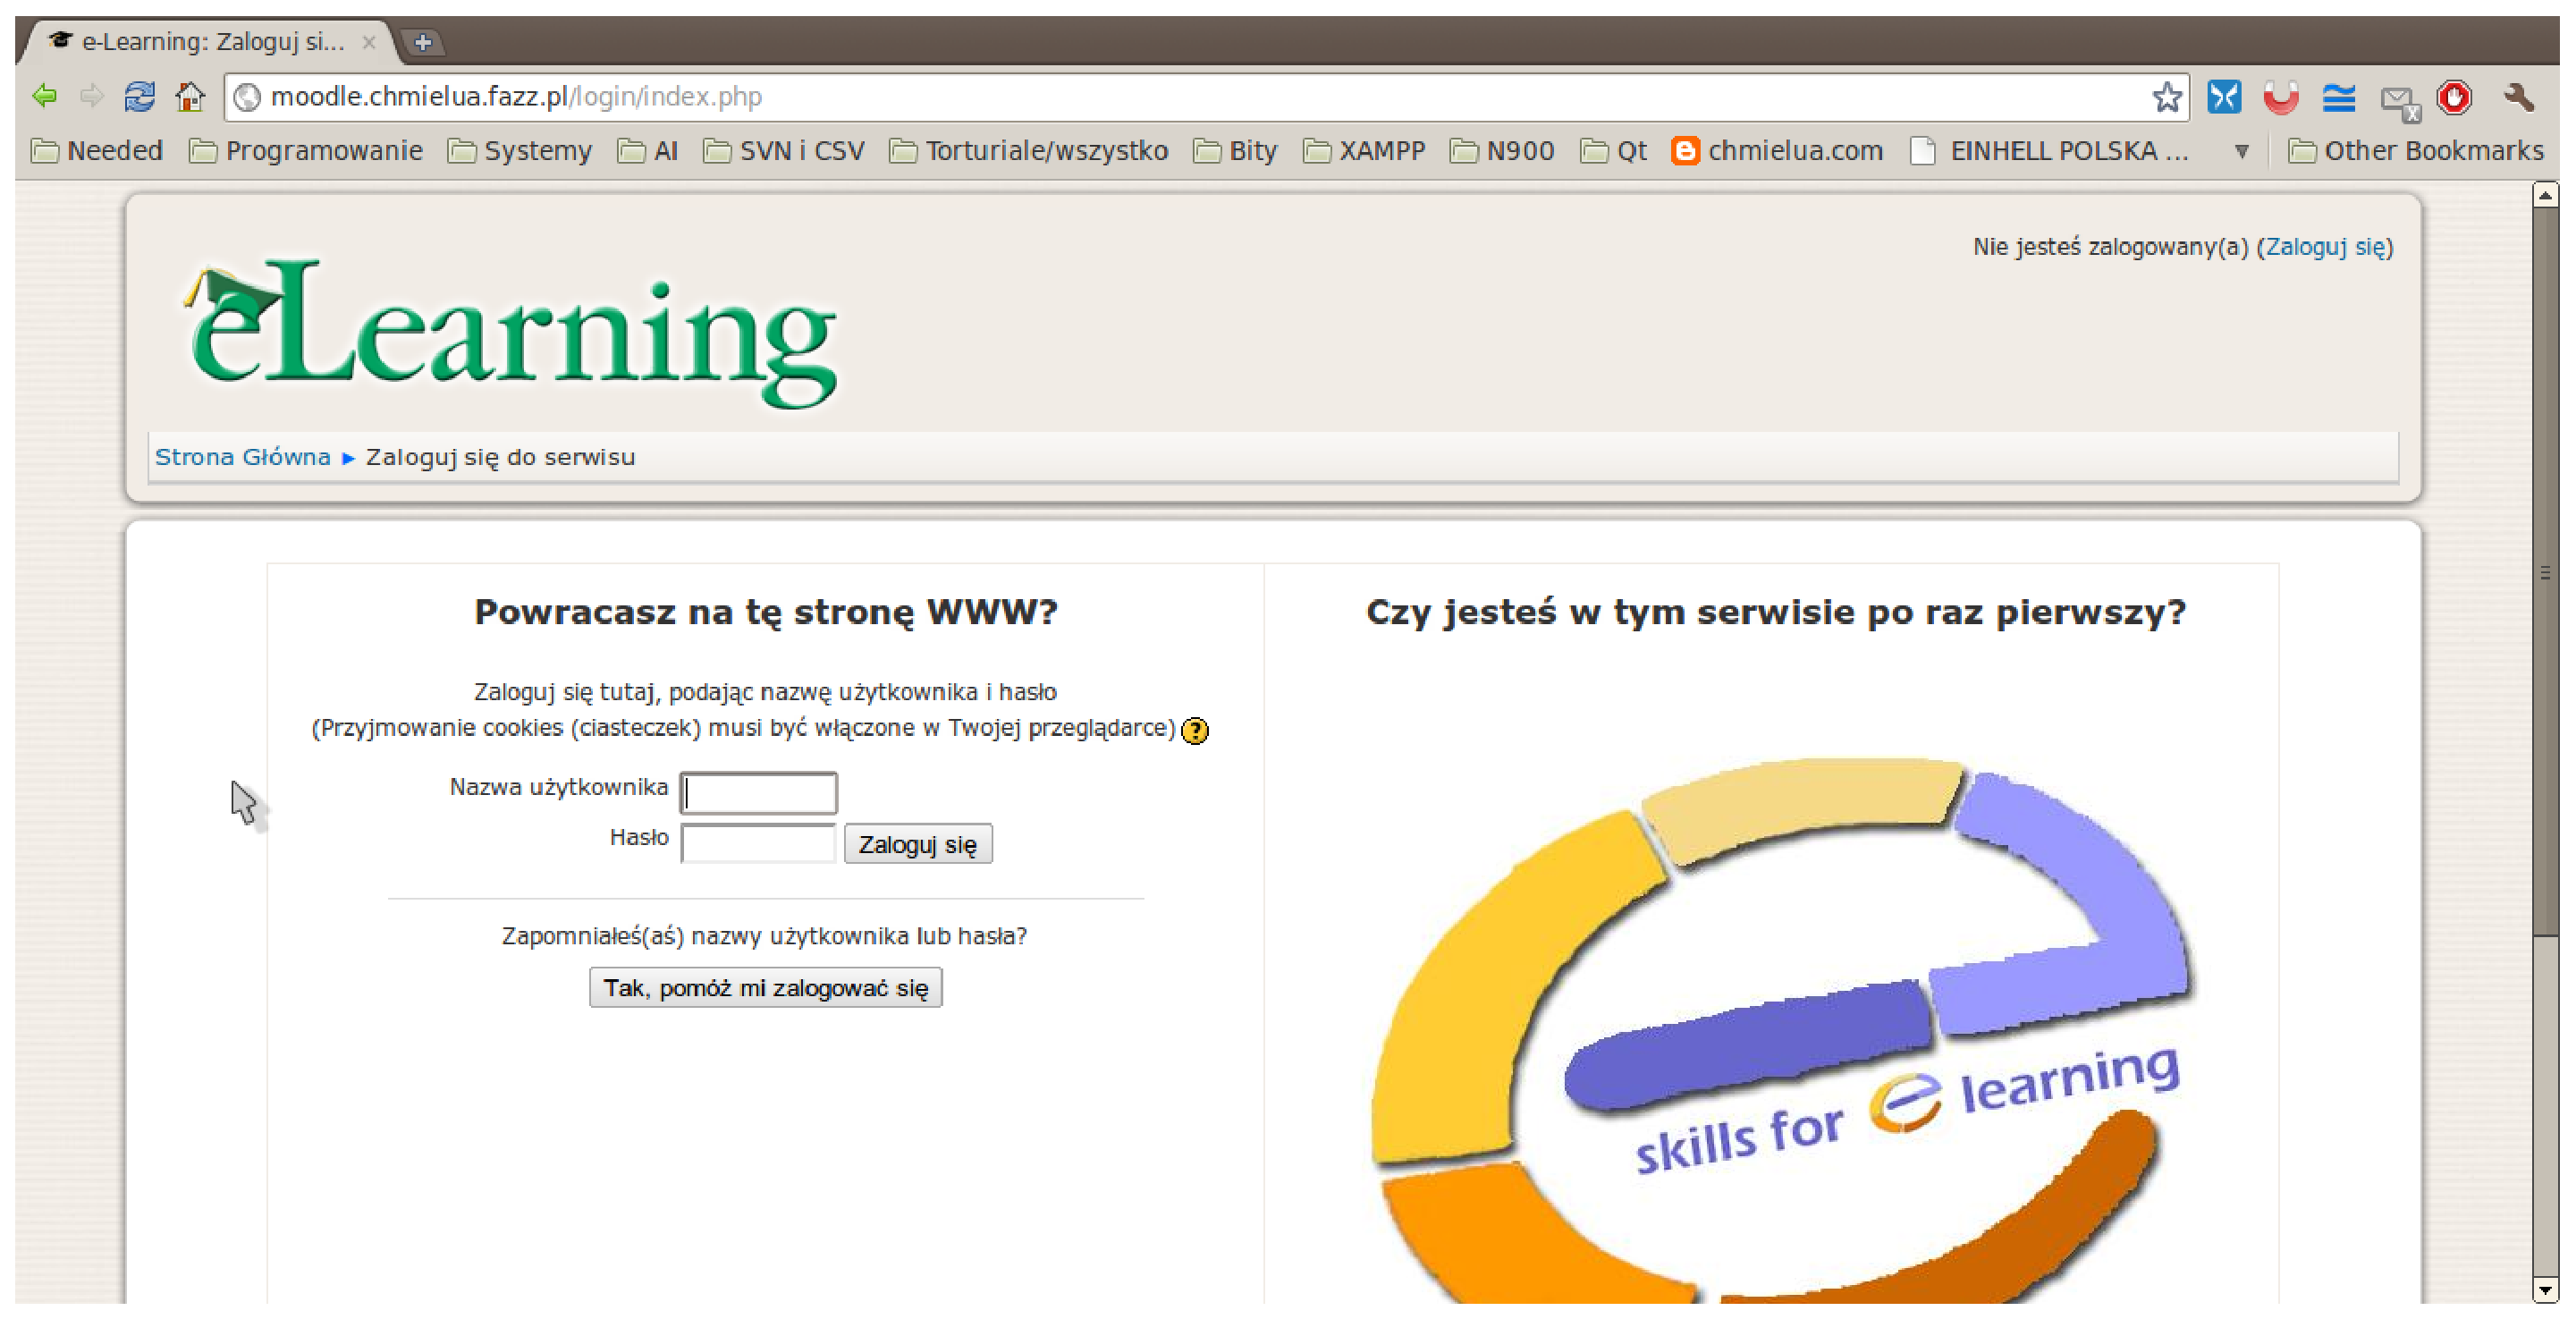
\includegraphics[width=1\textwidth]{projekt_sys//rys//logowanie.eps}
\end{figure}
Gdzie w przypadku braku konta, należy skorzystać z opcji \textit{Zacznij teraz od utworzenia nowego konta} rys. \ref{rys:nowy}.
\begin{figure}[!h]
	\centering
		\caption{Załorzenie nowego konta} \label{rys:nowy}
		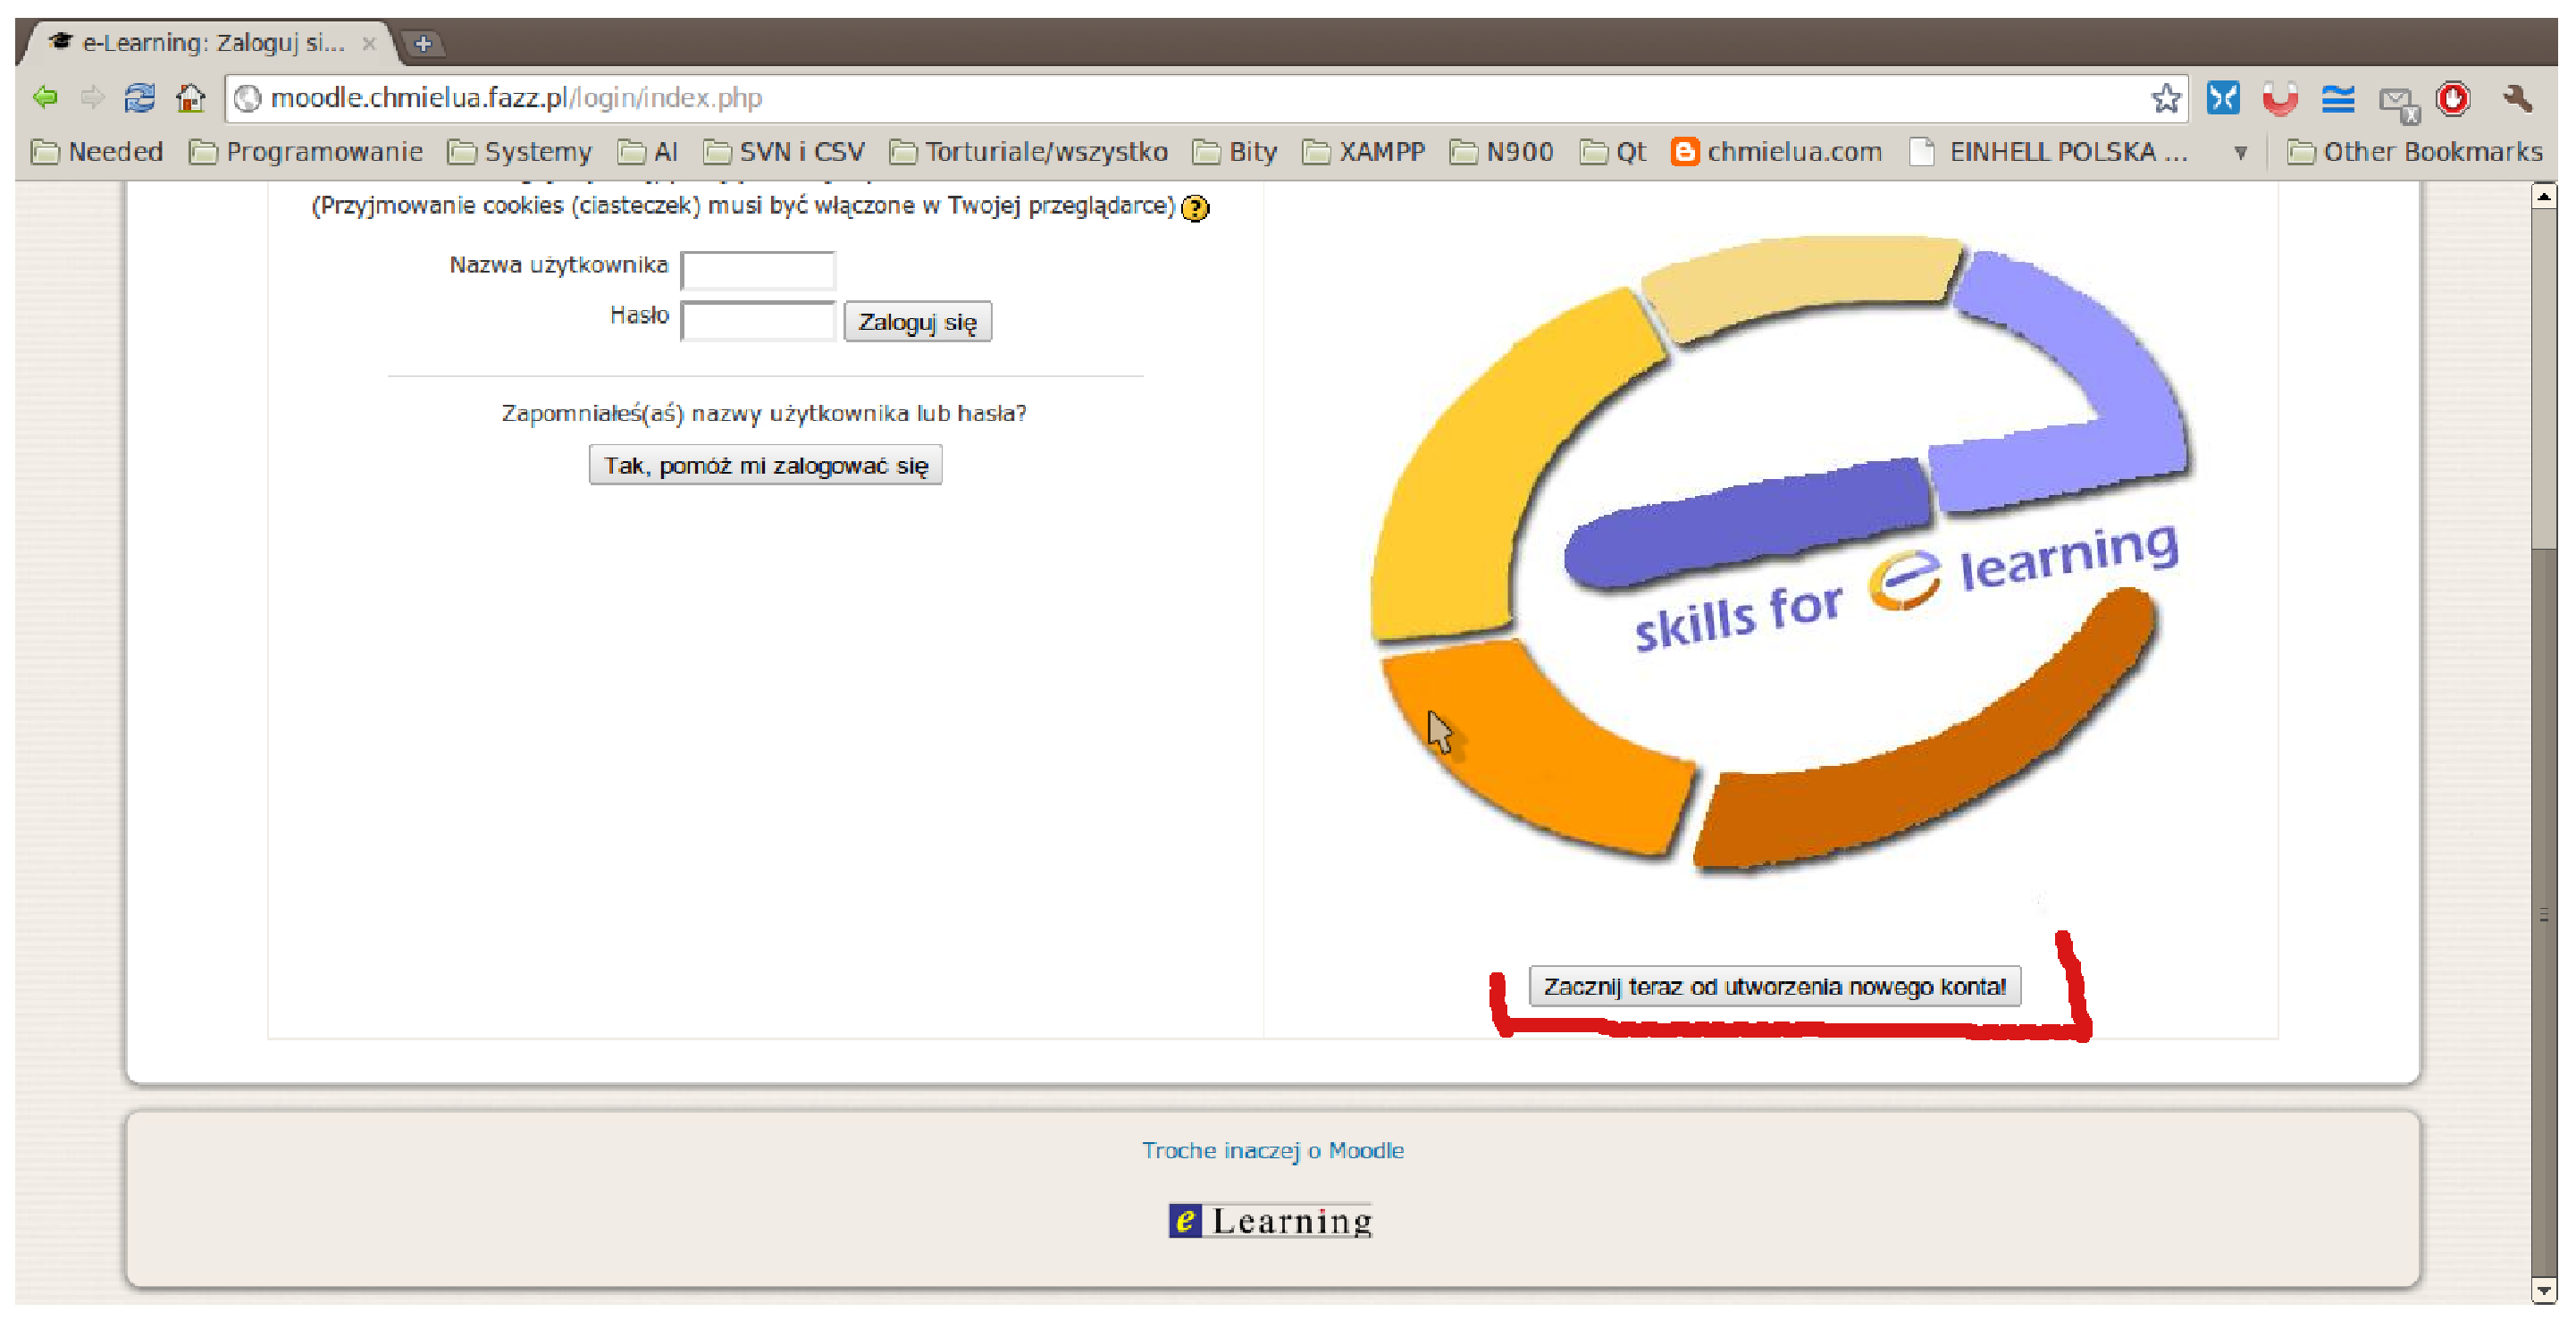
\includegraphics[width=1\textwidth]{projekt_sys//rys//nowy_user.eps}
\end{figure}
Po nacisnięciu \textit{Zacznij teraz od utworzenia nowego konta} zostaniemy przniesieni pod adres \href{http://moodle.chmielua.fazz.pl/login/signup.php?}{\textit{http://moodle.chmielua.fazz.pl/login/signup.php?}} rys.\ref{rys:signup}.
\begin{figure}[!h]
	\centering
		\caption{Formularz rejestracyjny} \label{rys:signup}
		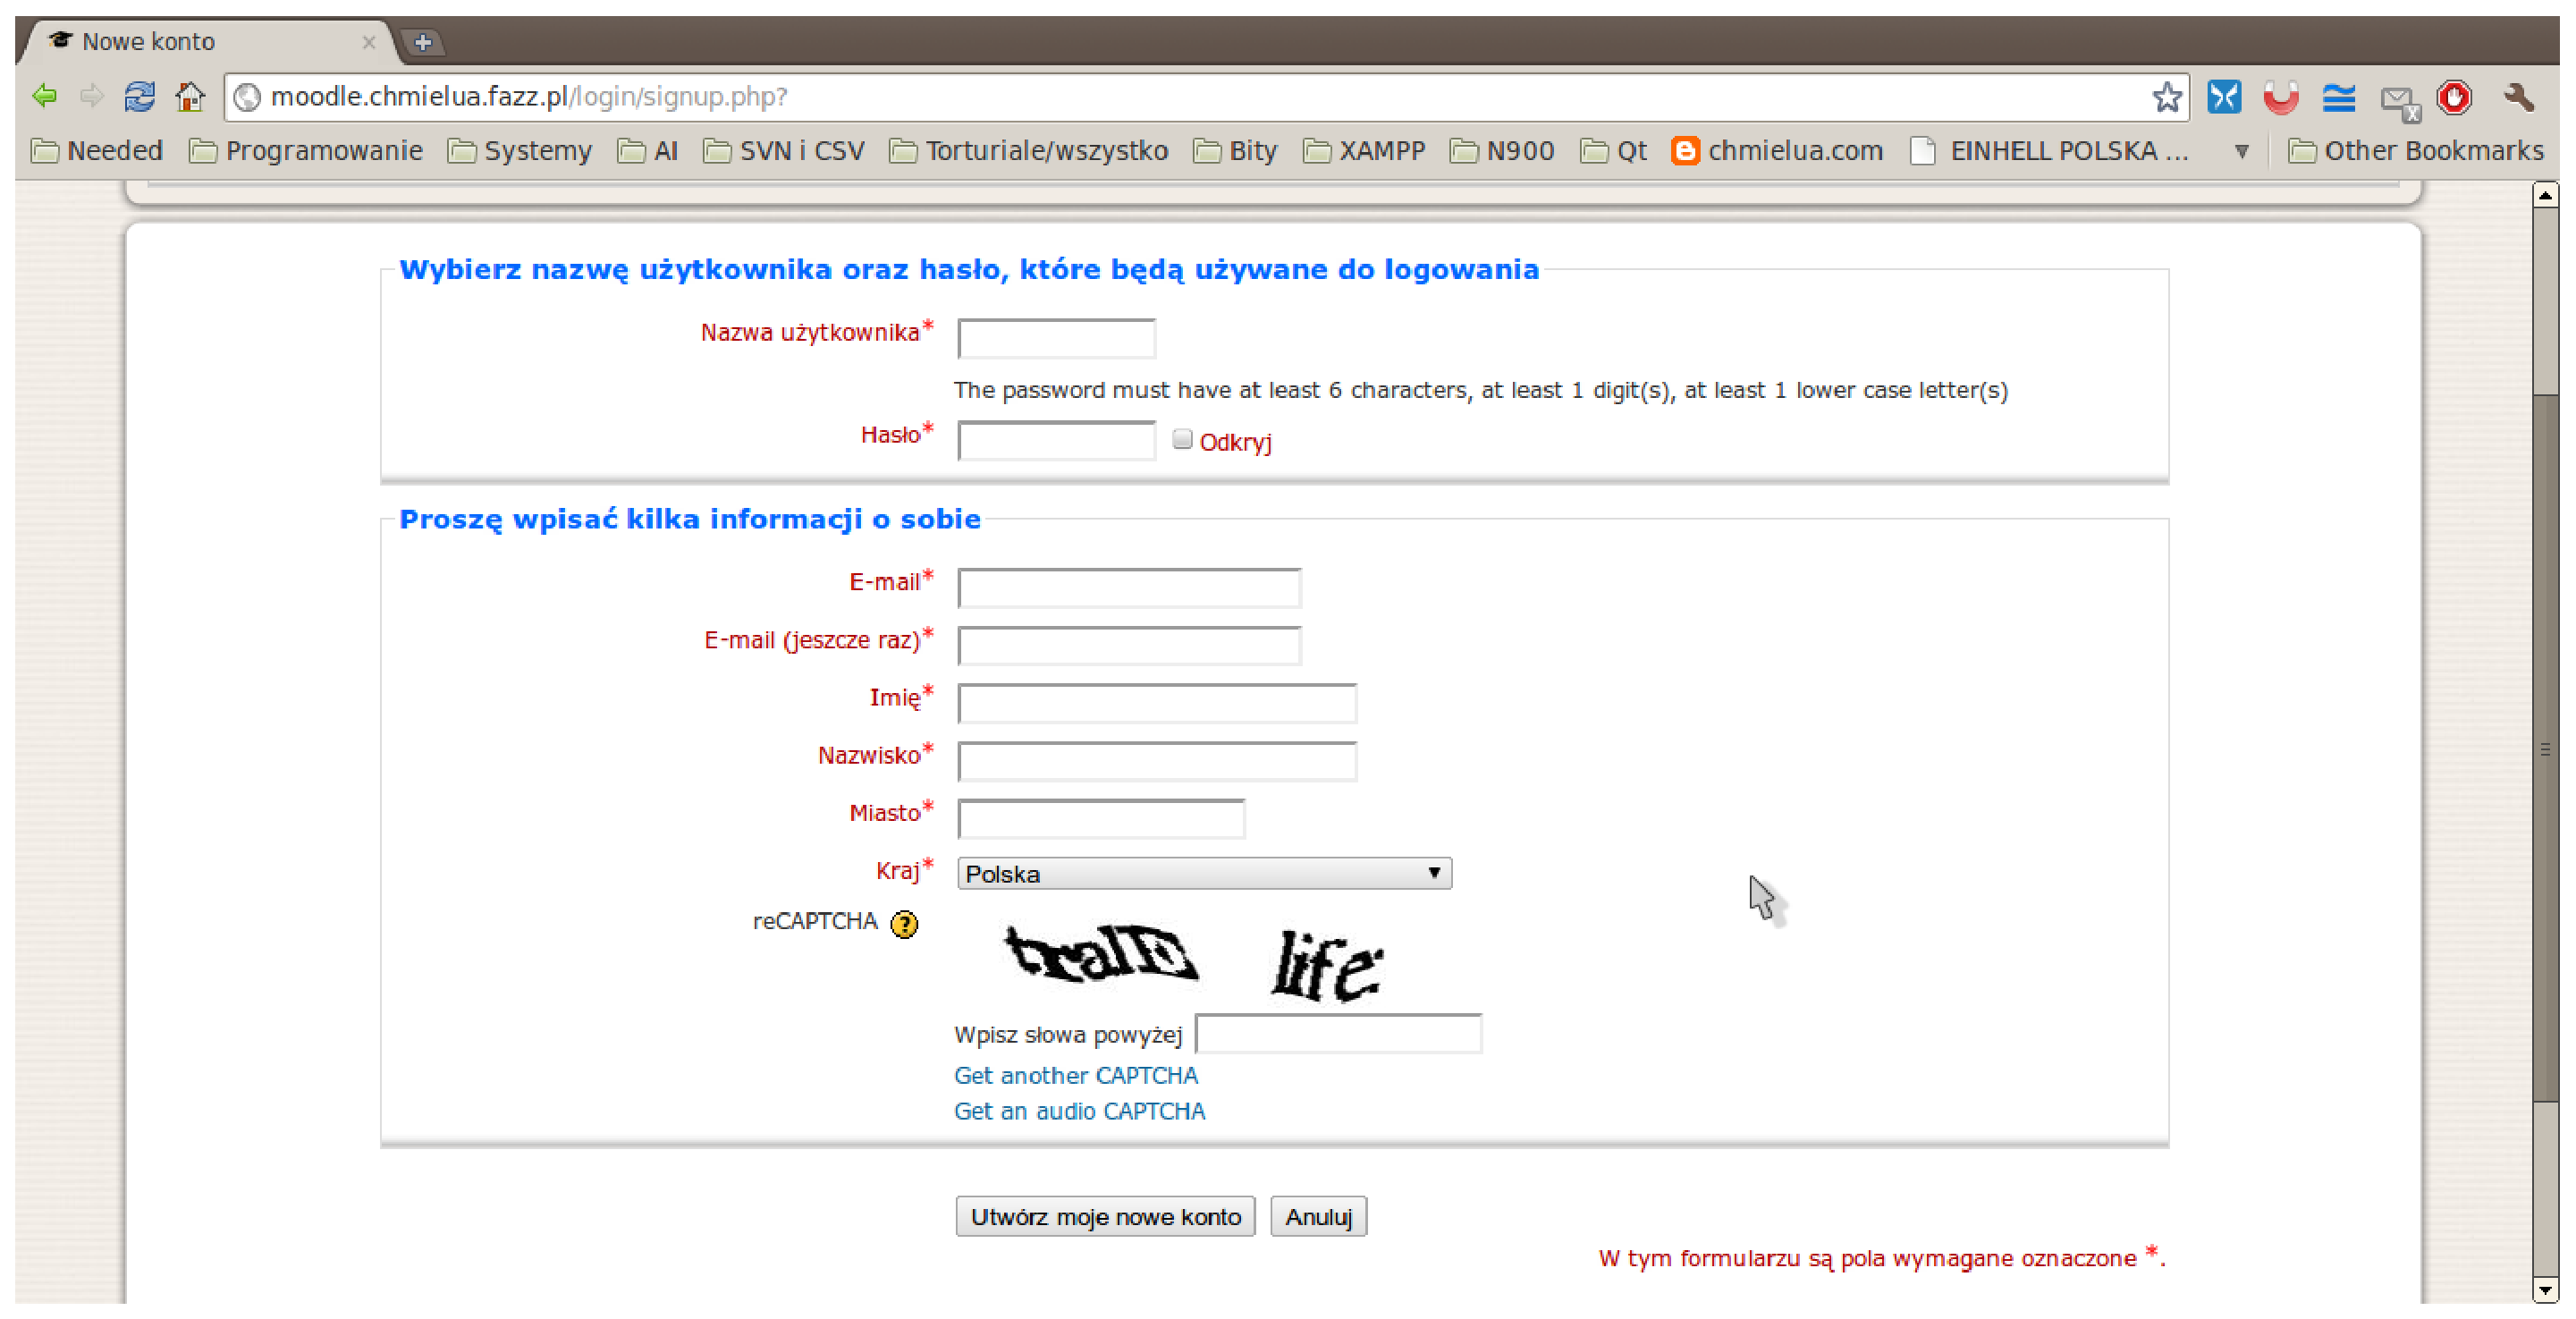
\includegraphics[width=1\textwidth]{projekt_sys//rys//rejestracja.eps}
\end{figure}
W celu wypełnienia formularza. Na jego podstawie zostanie utworzone nowe konto. Konto należy uwierzytelnić poprzez wejście w link wysłany w mailu na podany uprzednio adres. Dodawanie nowego użytkownika korzysta z zabezpieczenia reCAPTCHA, które chroni nas przed automatycznym tworzeniem nowych kont, które głównie są wykorzystywane do rozsyłania spamu. W przypadku gdy użytkownik zapomnie nazwę użytkownika lub hasło. Należy skorzystać z opcji \textit{Tak, pomóż mi zalogować się}. Po skorzystaniu z tej opcji zostajemy przeniesieni pod adres \href{http://moodle.chmielua.fazz.pl/login/forgot_password.php}{\textit{http://moodle.chmielua.fazz.pl/login/forgot\_password.php}} rys.\ref{rys:lost_pass}
\begin{figure}[!h]
	\centering
		\caption{Zapomniane hasło} \label{rys:lost_pass}
		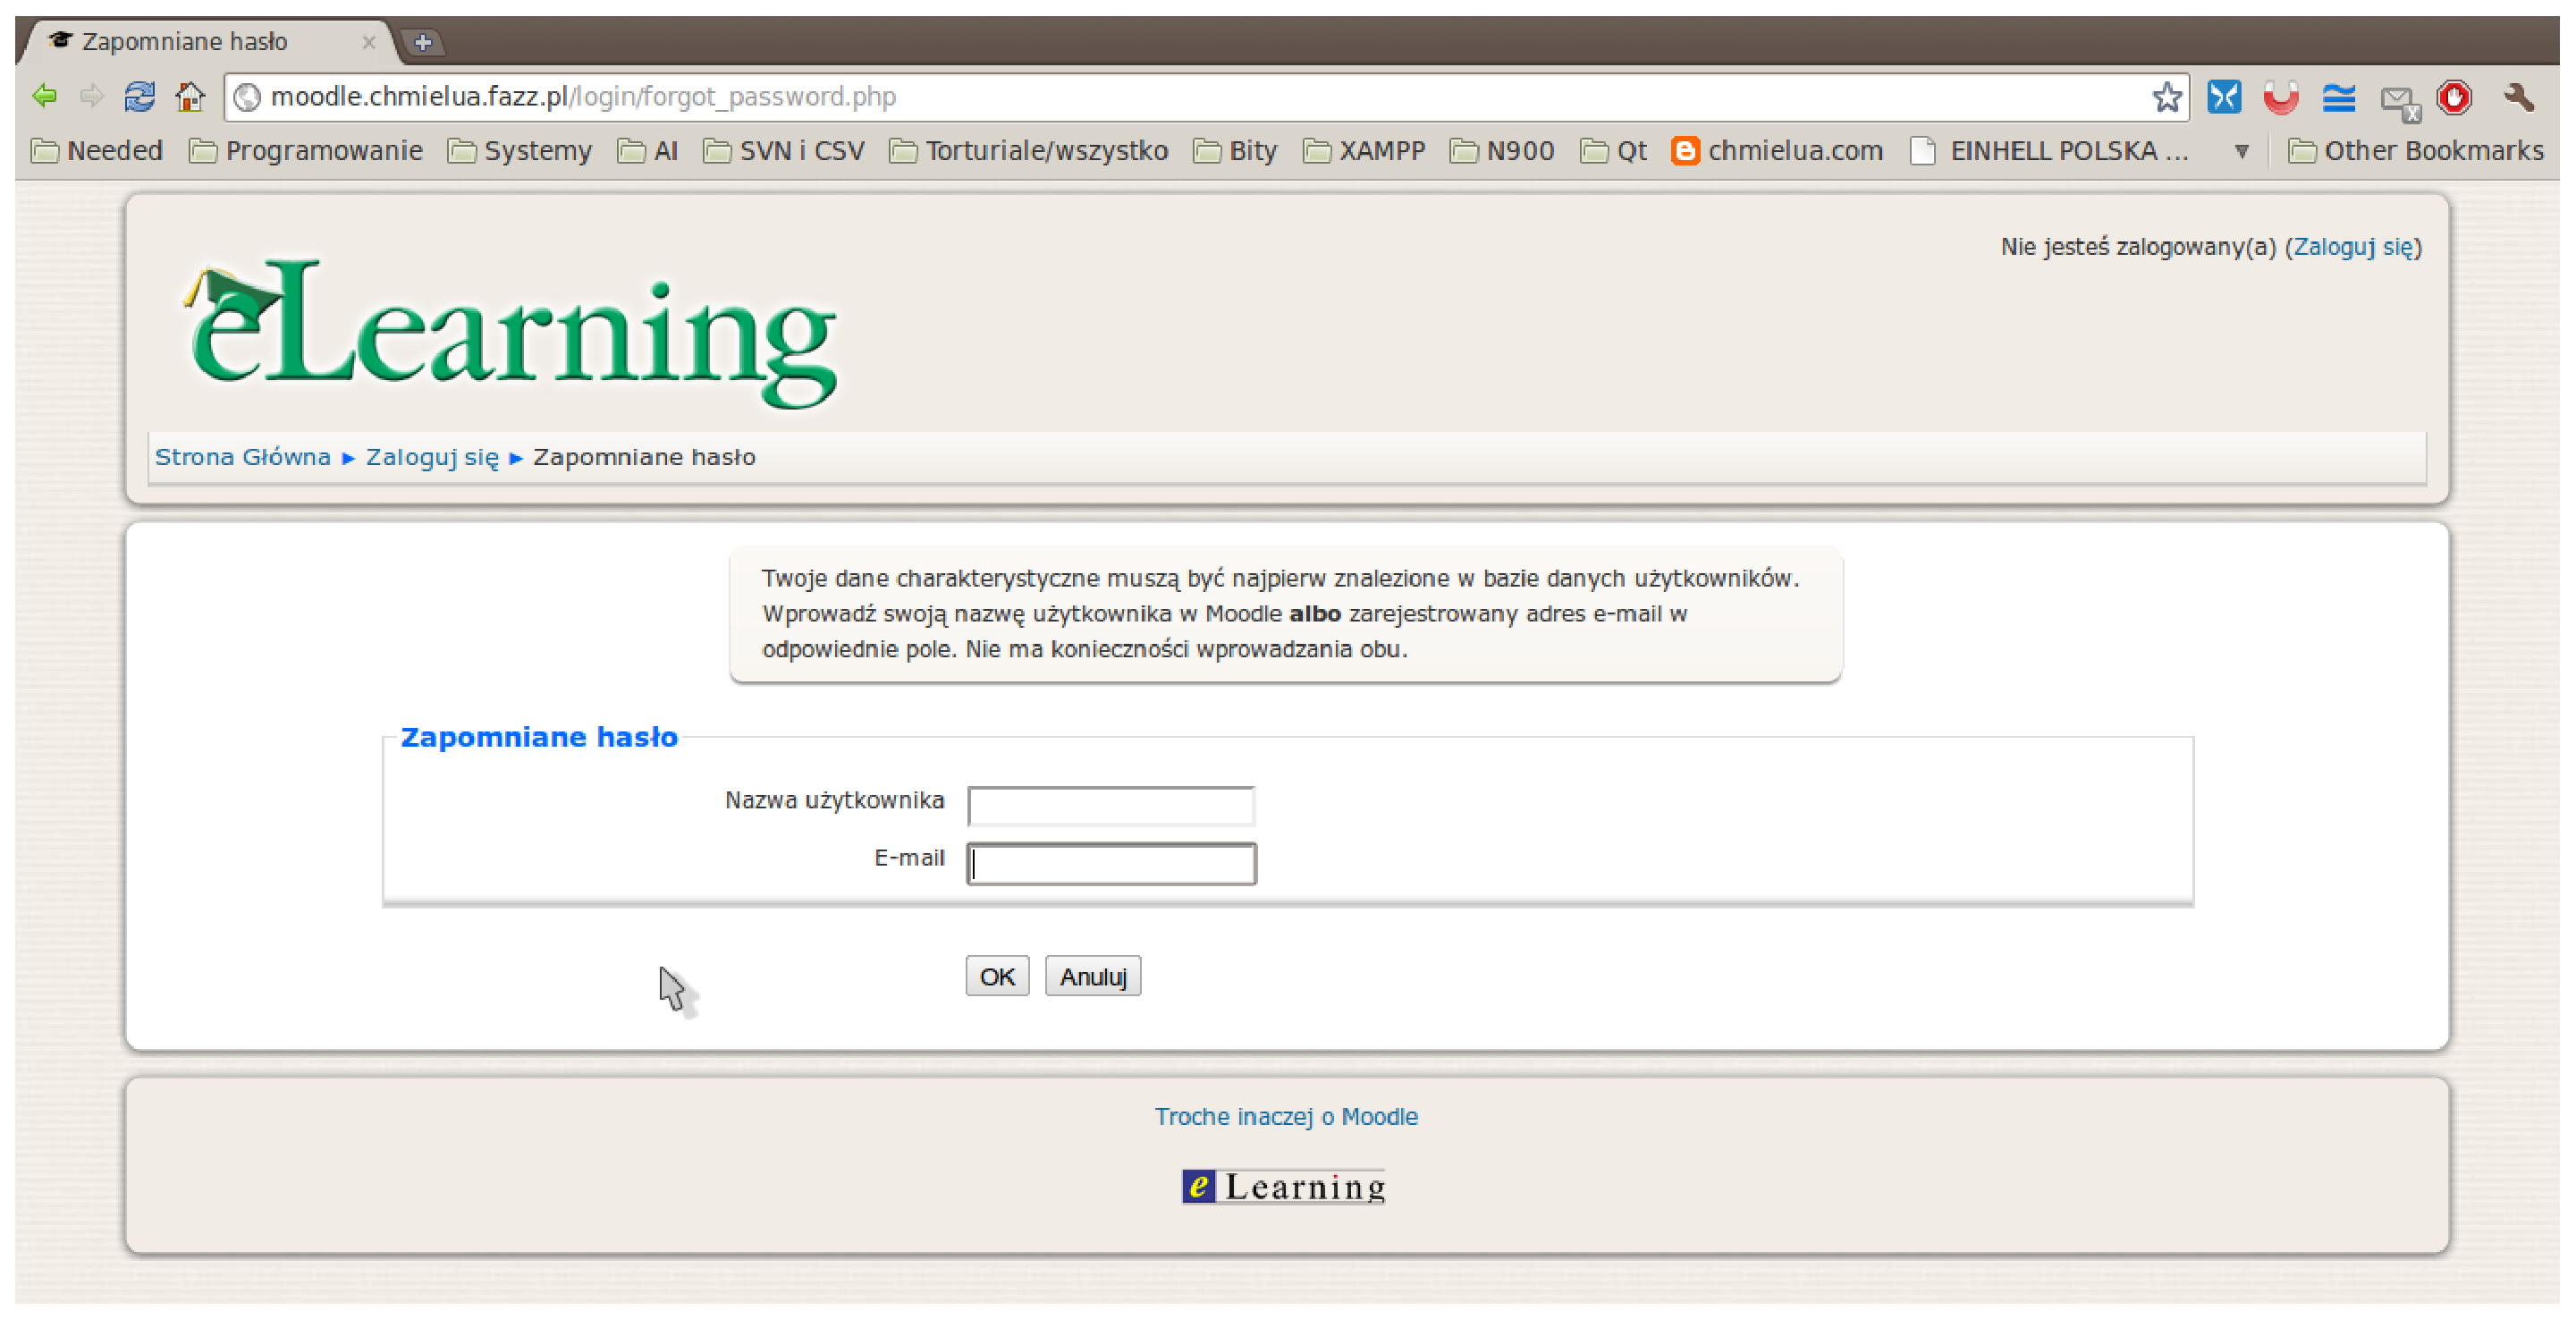
\includegraphics[width=1\textwidth]{projekt_sys//rys//lost_pass.eps}
\end{figure}
Na stronie należy wypełnić jedno z dwóch pól i wcisnąć \textit{OK}. Zostanie wysłana wiadomość, gdzie aby potwierdzić i otrzymać nowe hasło za pośrednictwem poczty elektronicznej, nalezy przejść na podana pod spodem stronę. Strona ta powinna wyglądać tak jak na rys.\ref{rys:new_pass}.
\begin{figure}[!h]
	\centering
		\caption{Automatyczna generacja nowego hasła} \label{rys:new_pass}
		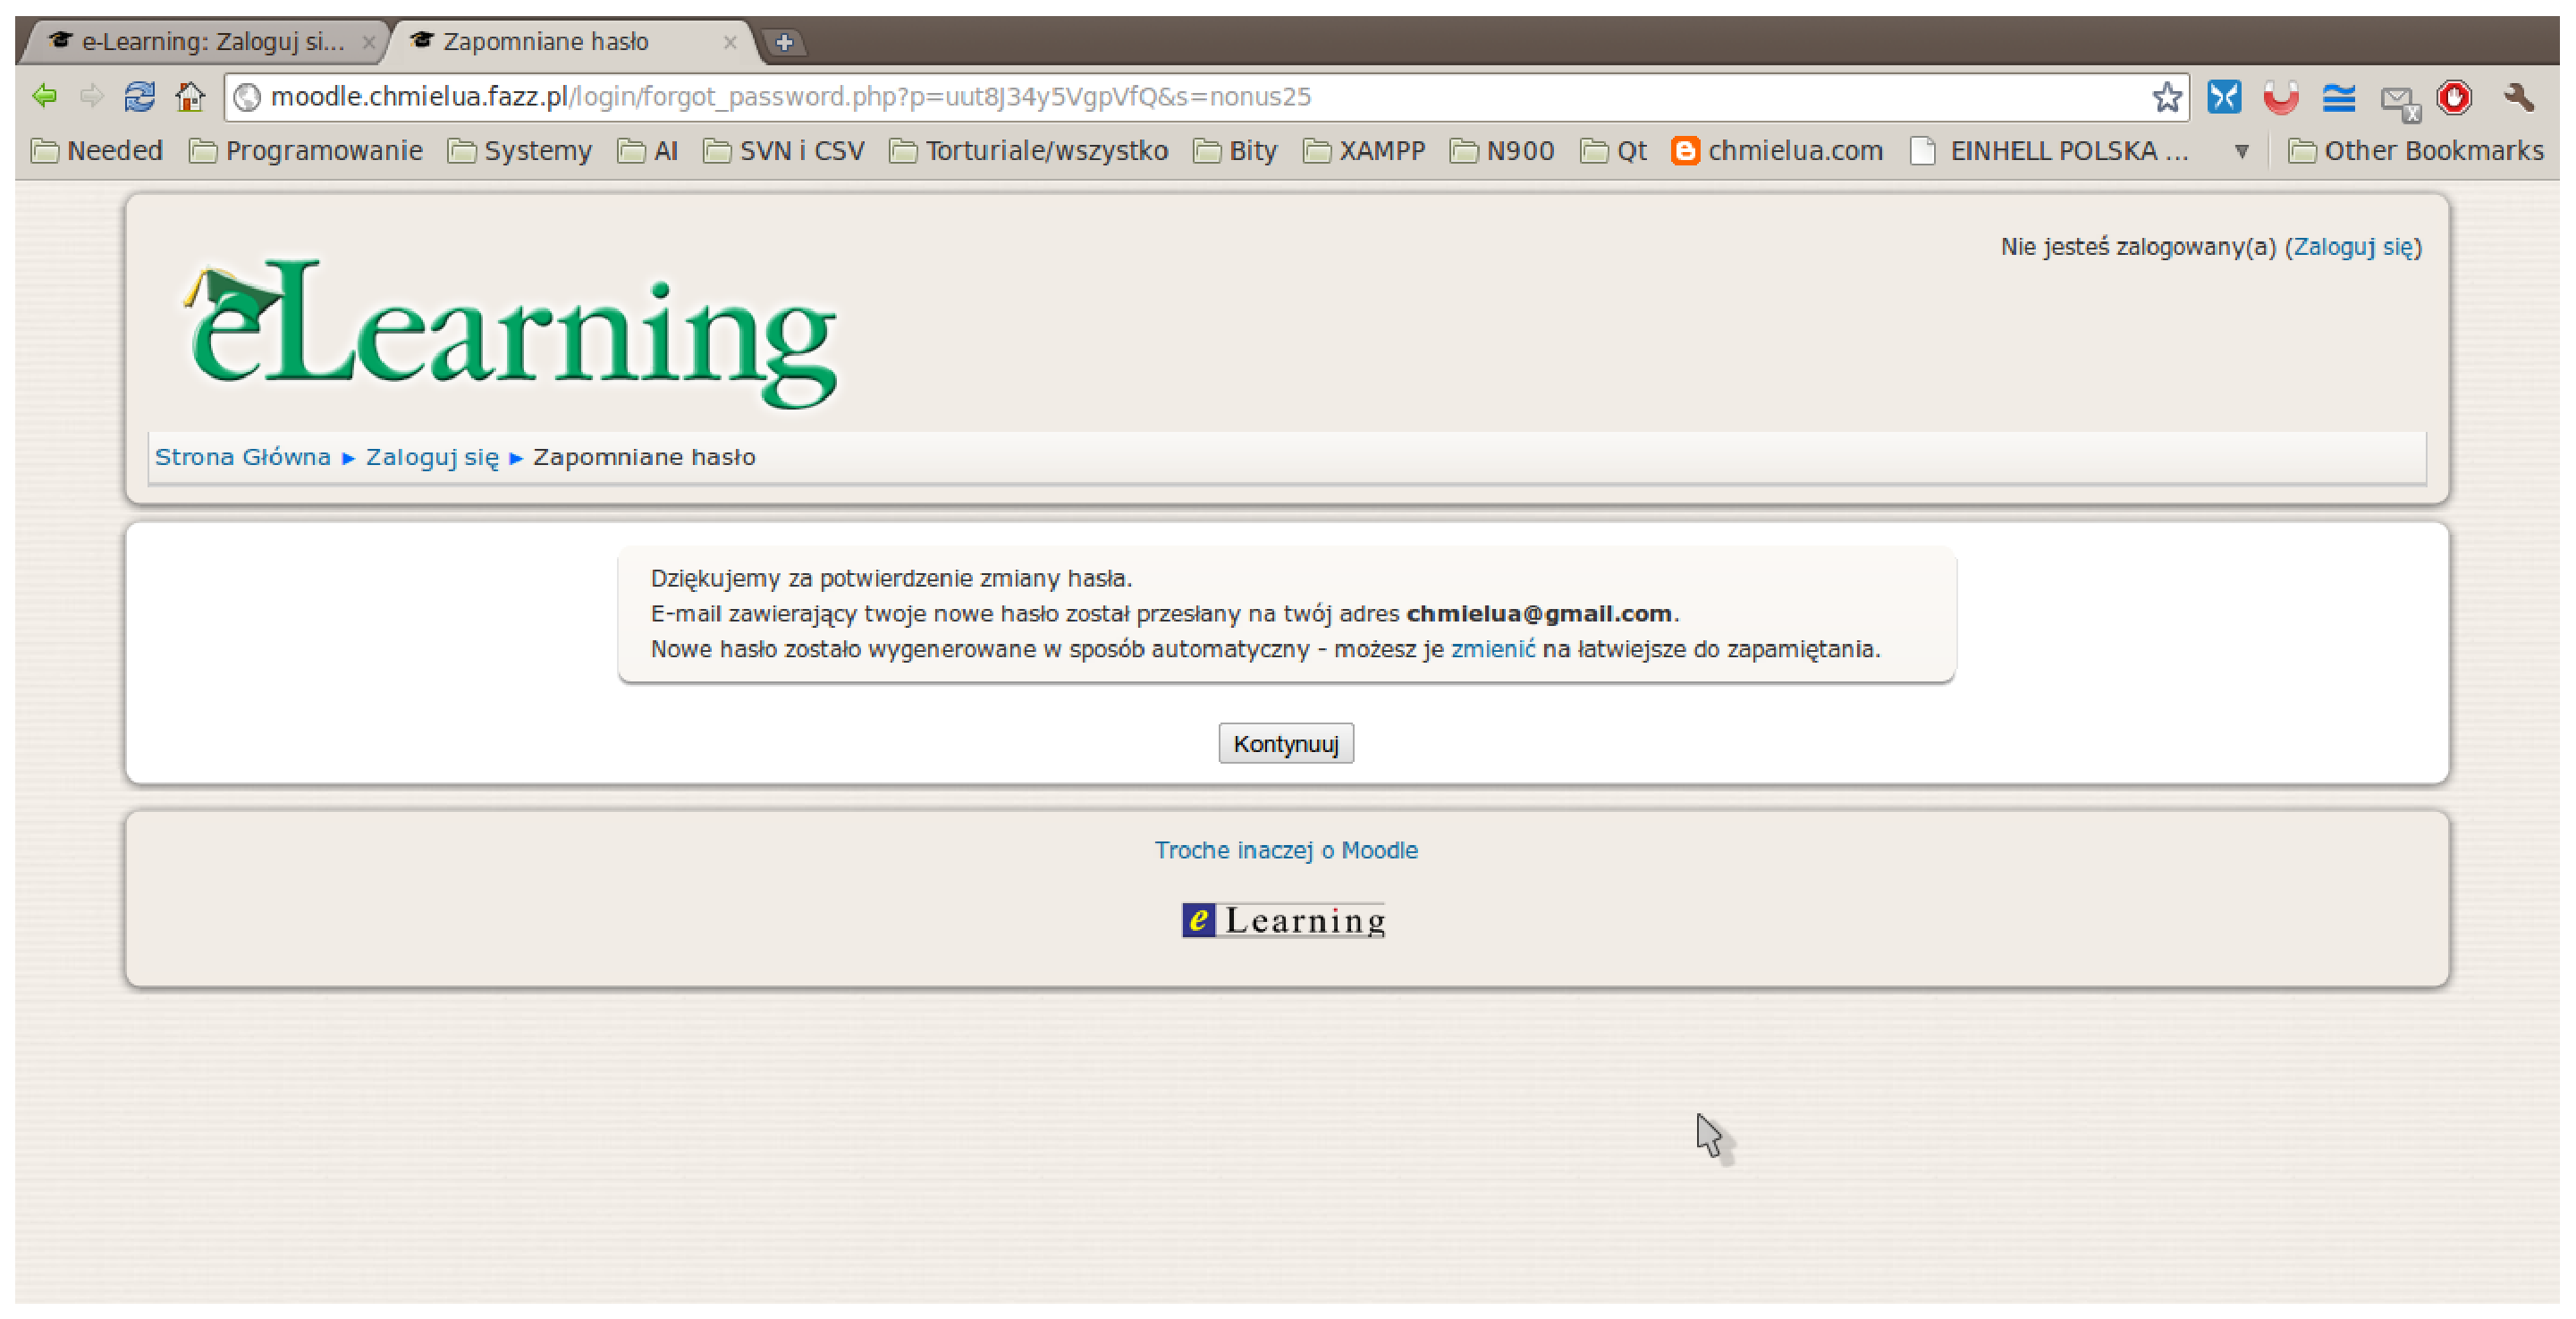
\includegraphics[width=1\textwidth]{projekt_sys//rys//nowe_haslo.eps}
\end{figure}
Po wciśnięciu kontynuuj zostanie ponownie wyslana wiadomość do nas. Wiadomość ta będzie zawierać nowe hasło, nazwę użytkownika i link do zmiany wygenerowanego hasła. Gdy przejdziemy do strony odpowiedającej za zmiane hasła\ref{rys:zmien_haslo} należy podać hasło, które zostało do nas wysłane, a następnie podać swoje własne nowe hasło. 
\begin{figure}[!h]
	\centering
		\caption{Ręczna zmiana hasła} \label{rys:zmien_haslo}
		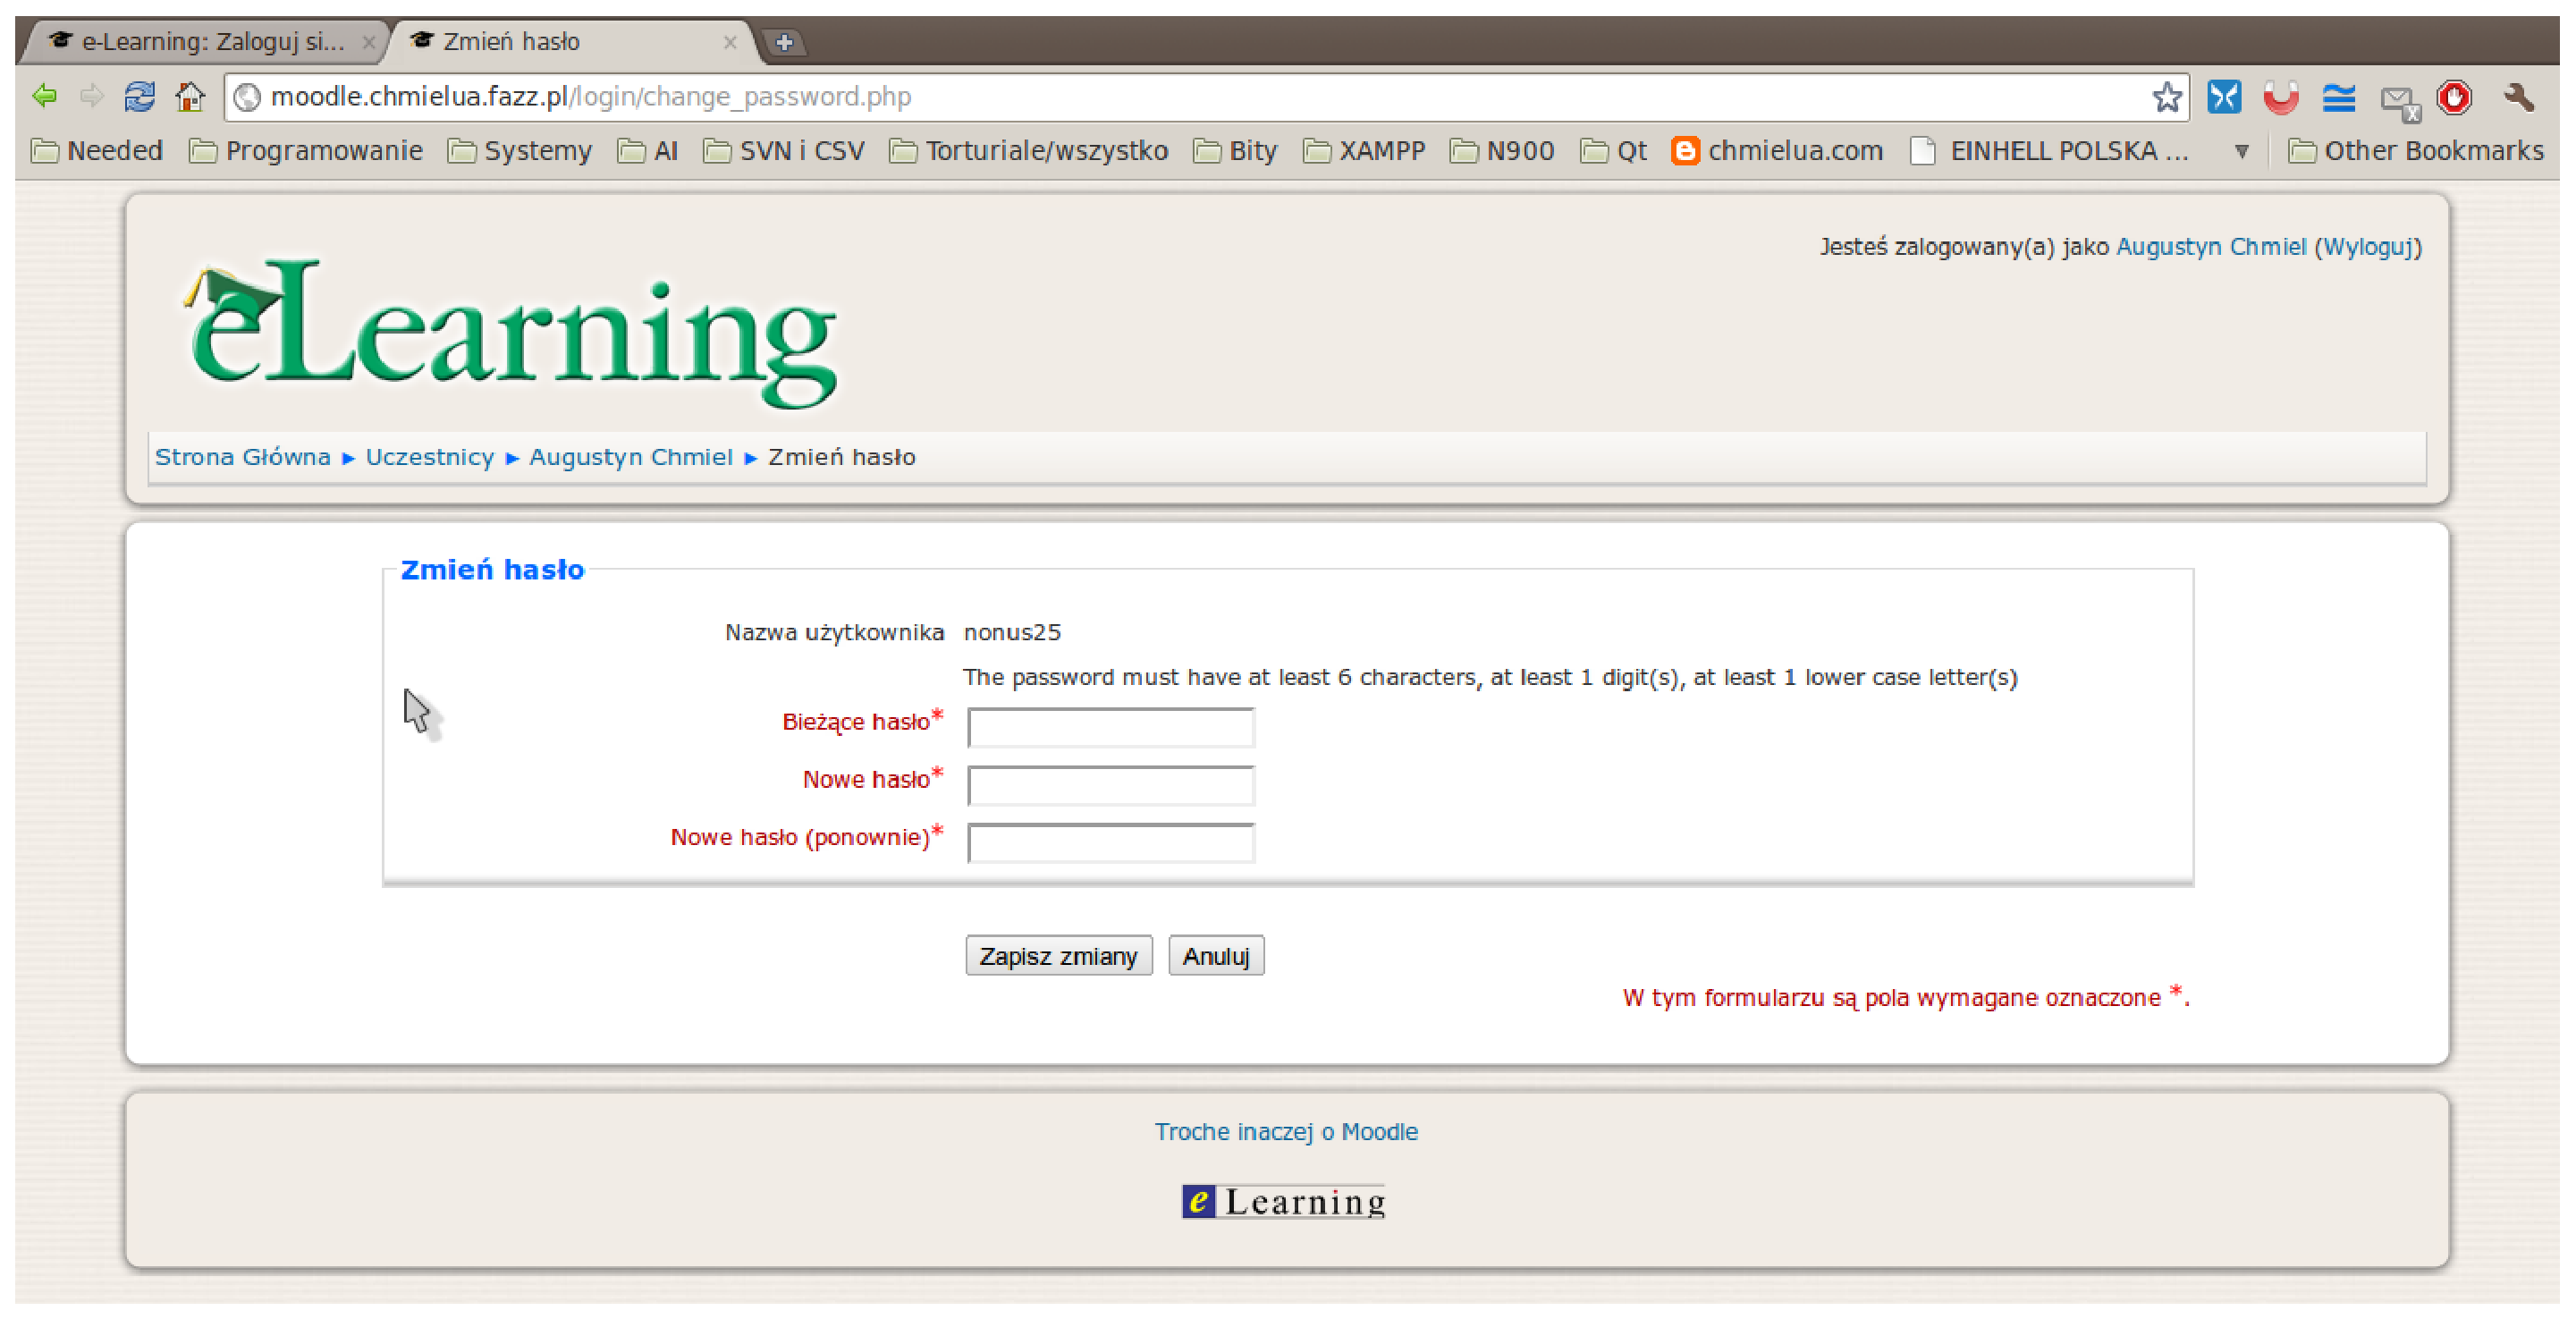
\includegraphics[width=1\textwidth]{projekt_sys//rys//zmiana_hasla.eps}
\end{figure}
Przy istniejącym kącie i po udanej próbie logowania jesteśmy wstanie zobaczyć strone główną witryny \href{http://moodle.chmielua.fazz.pl/}{\textit{http://moodle.chmielua.fazz.pl/}} rys. \ref{rys:glowna}
\begin{figure}[!h]
	\centering
		\caption{Strona główna} \label{rys:glowna}
		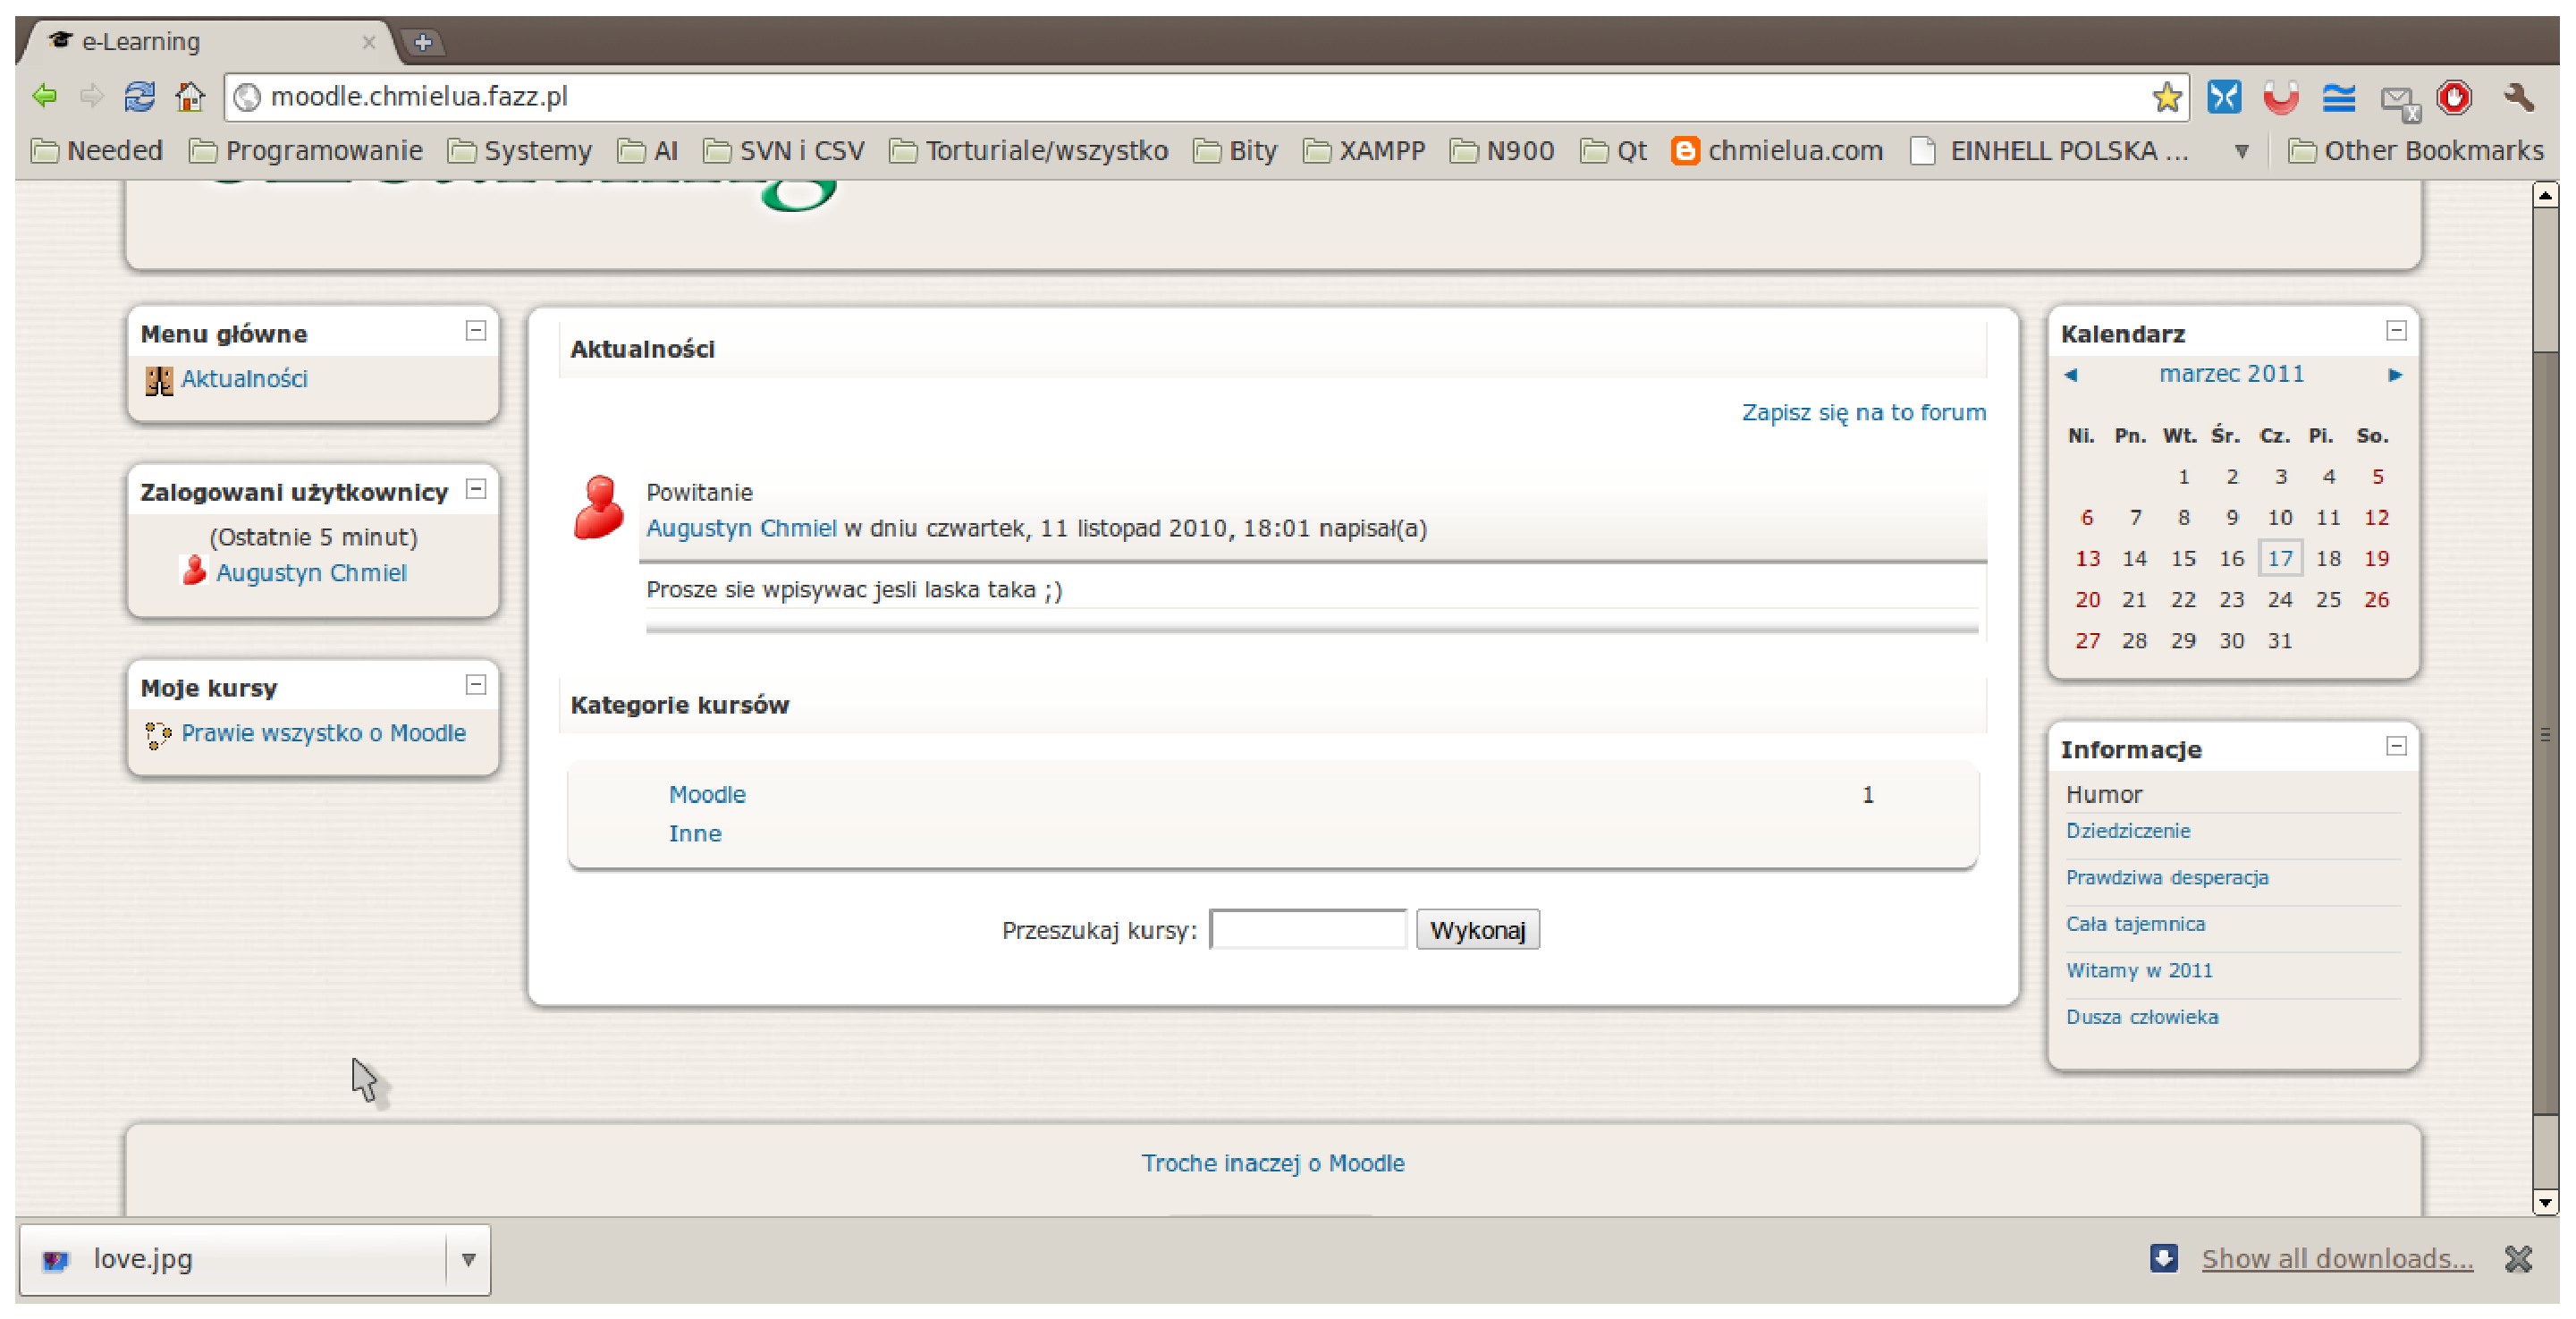
\includegraphics[width=1\textwidth]{projekt_sys//rys//glowna.eps}
\end{figure}
Na stronie głównej znajdują się podstawowe informacje takie jak Aktualności, Uczestnicy, Zalogowani użytkownicy, Kategorie kursów, Kalendarz i Humor zaciągnięty ze strony \href{http://demotywatory.pl/}{\textit{http://demotywatory.pl/}} przy wykorzystaniu kanału RSS\footnote{RSS – umowna rodzina języków znacznikowych do przesyłania nagłówków wiadomości i nowości na wybranych przez użytkownika RSS stronach.}. Następnie w bloku o tytule \textit{Kategorie kursów} znajdują się dwie kategorie \textit{Moodle} i \textit{Inne} co widać dokladnie na rys. \ref{rys:glowna}. Kategoria Moodle zawiera kurs który nosi nazwę \textit{Prawie wszystko o Moodle} rys. \ref{rys:kurs}
\begin{figure}[!h]
	\centering
		\caption{Kategorja Moodle} \label{rys:kurs}
		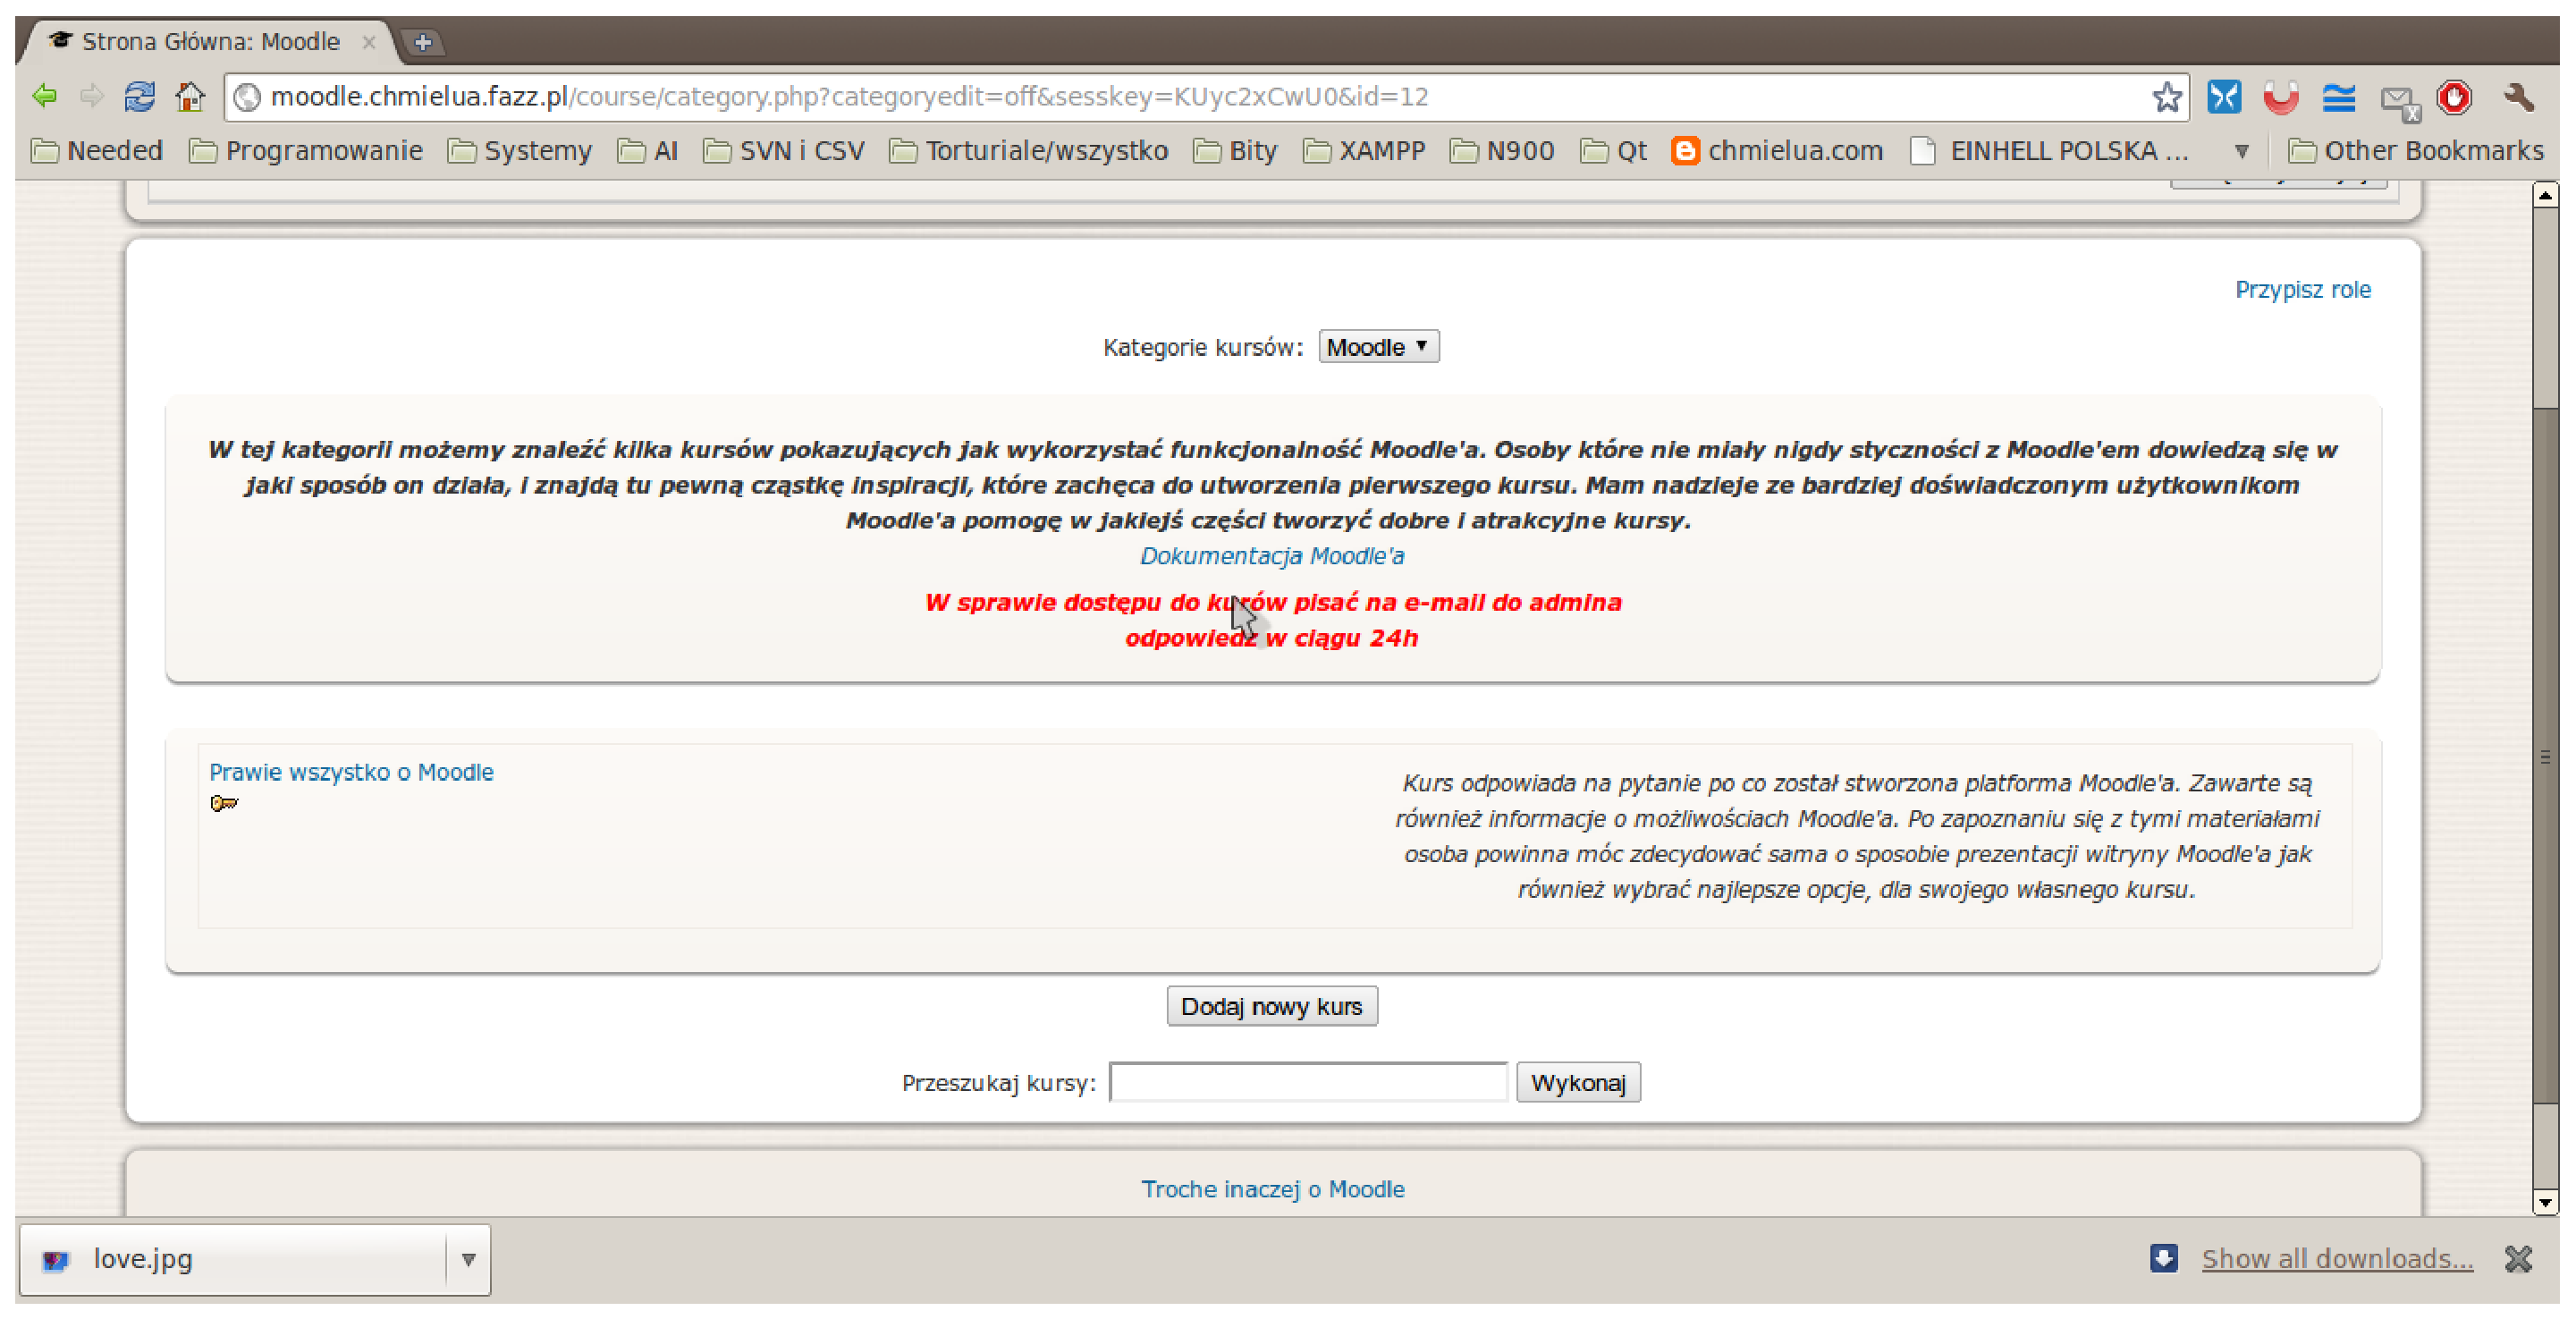
\includegraphics[width=1\textwidth]{projekt_sys//rys//kurs.eps}
\end{figure}
\begin{figure}[!h]
	\centering
		\caption{Kurs: Prawie wszystko o Moodle} \label{rys:kurs_moodle}
		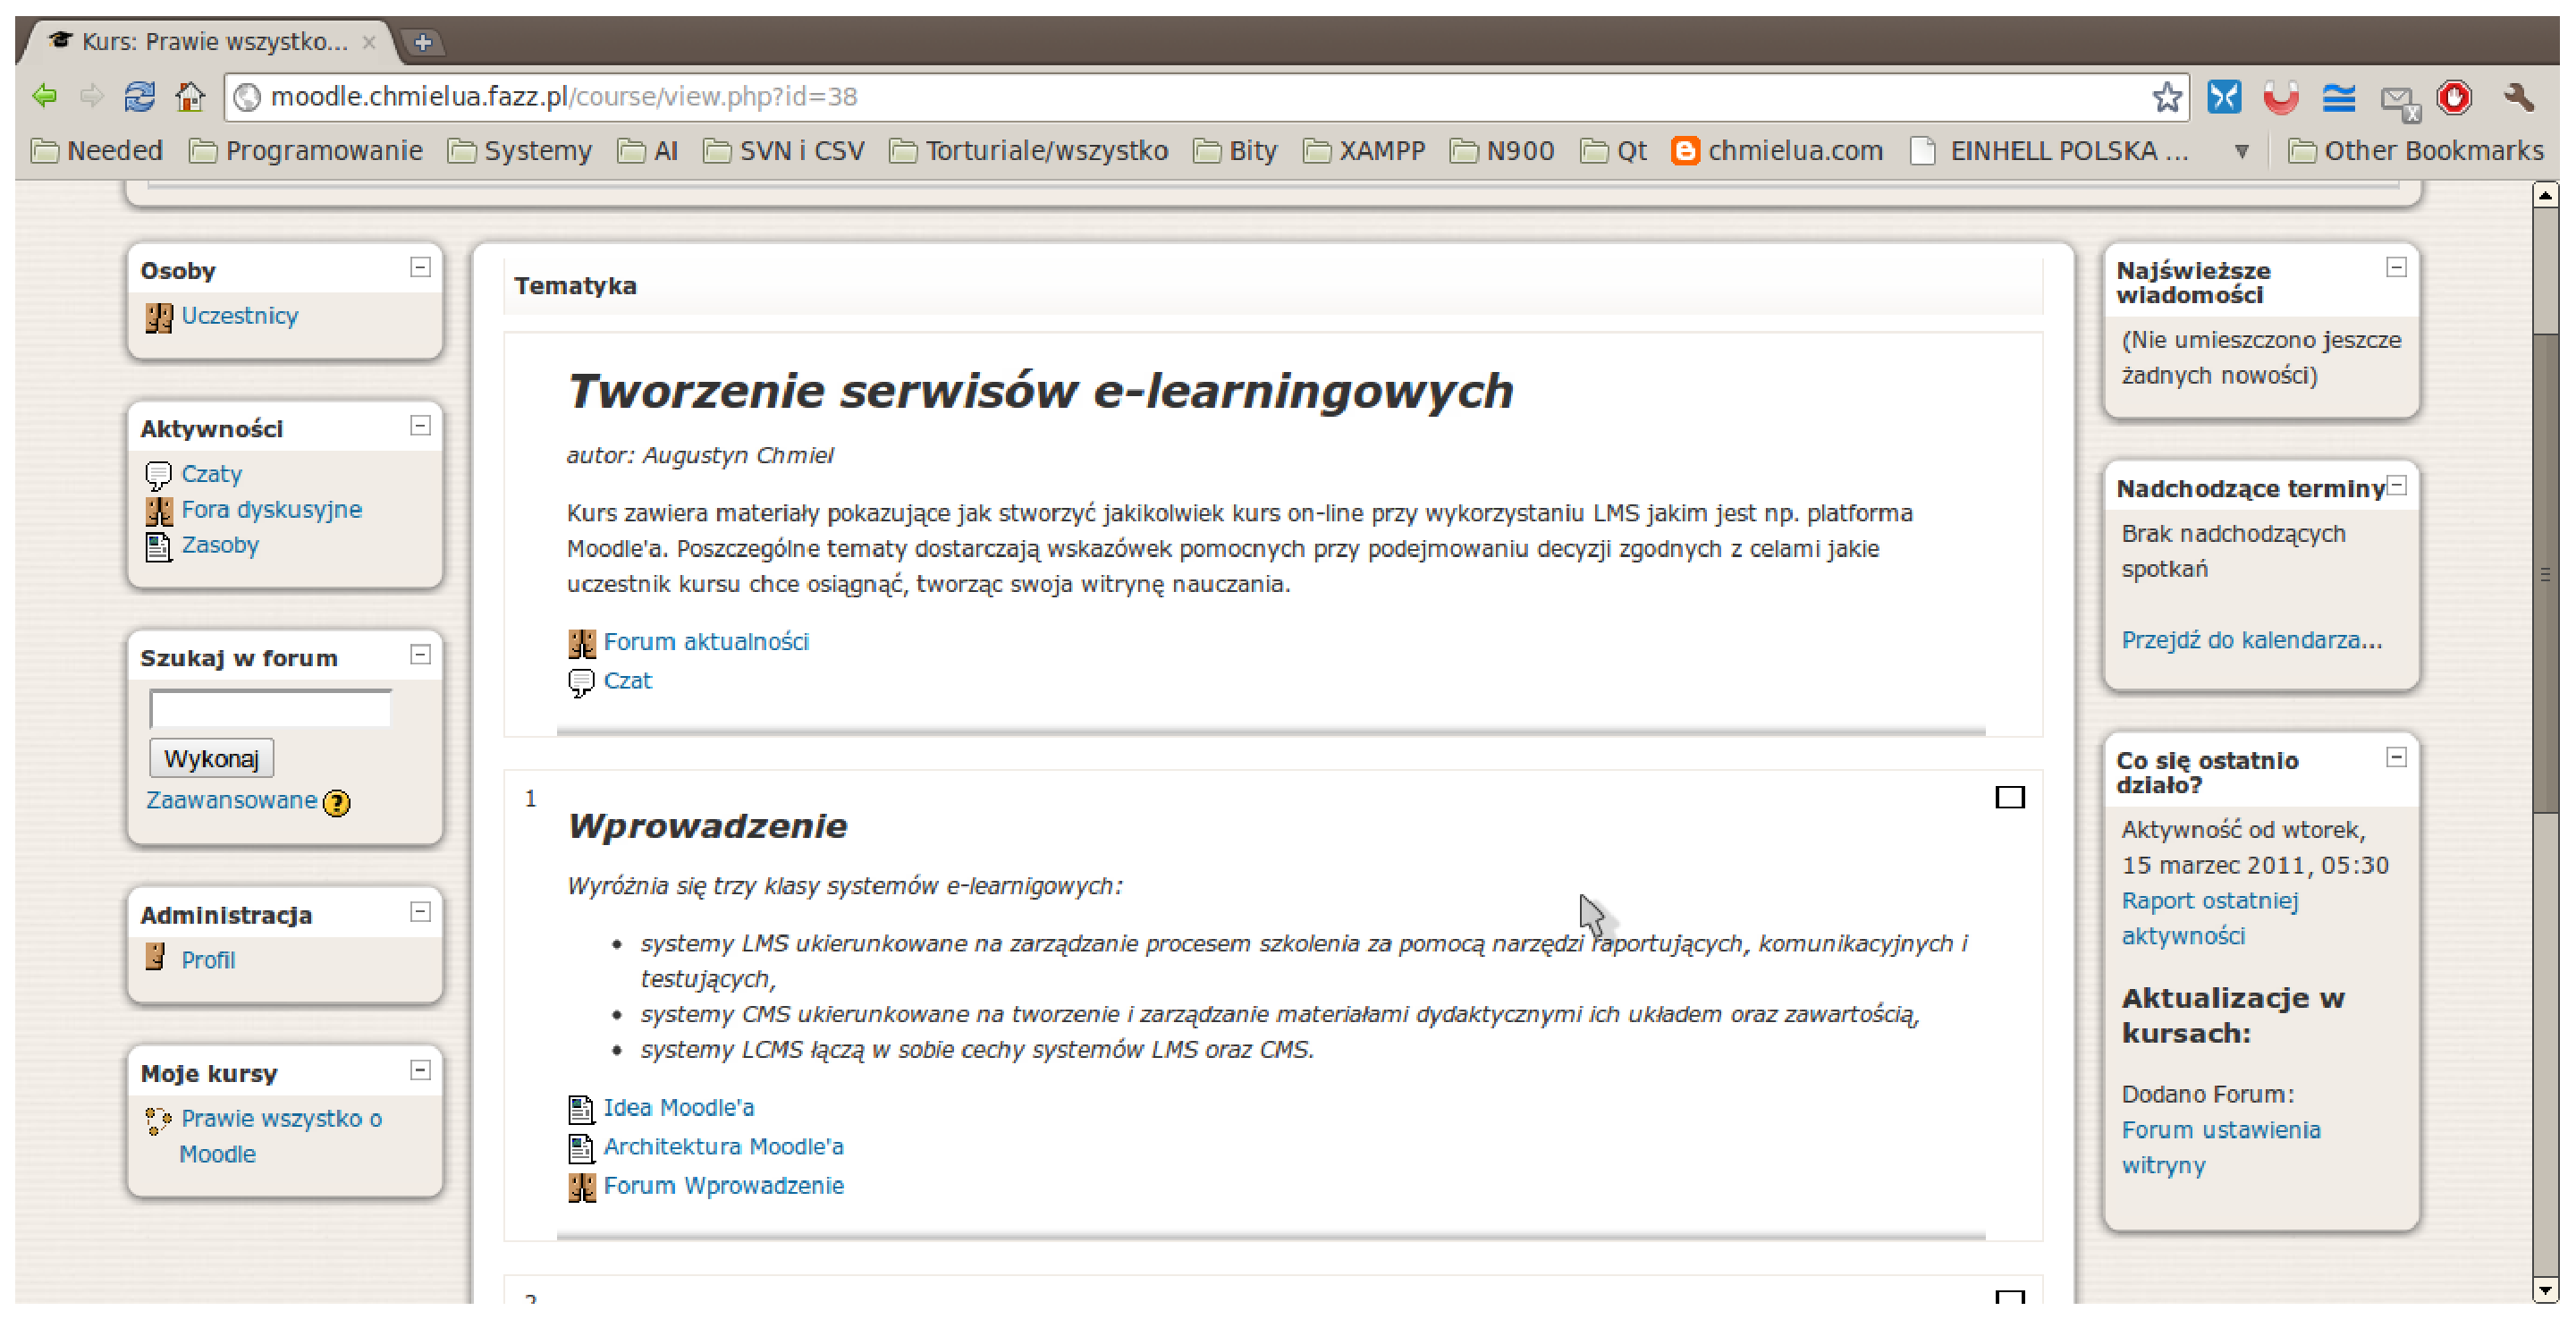
\includegraphics[width=1\textwidth]{projekt_sys//rys//kurs_moodle.eps}
\end{figure}
\begin{figure}[!h]
	\centering
		\caption{Kurs: Prawie wszystko o Moodle} \label{rys:kurs_moodle2}
		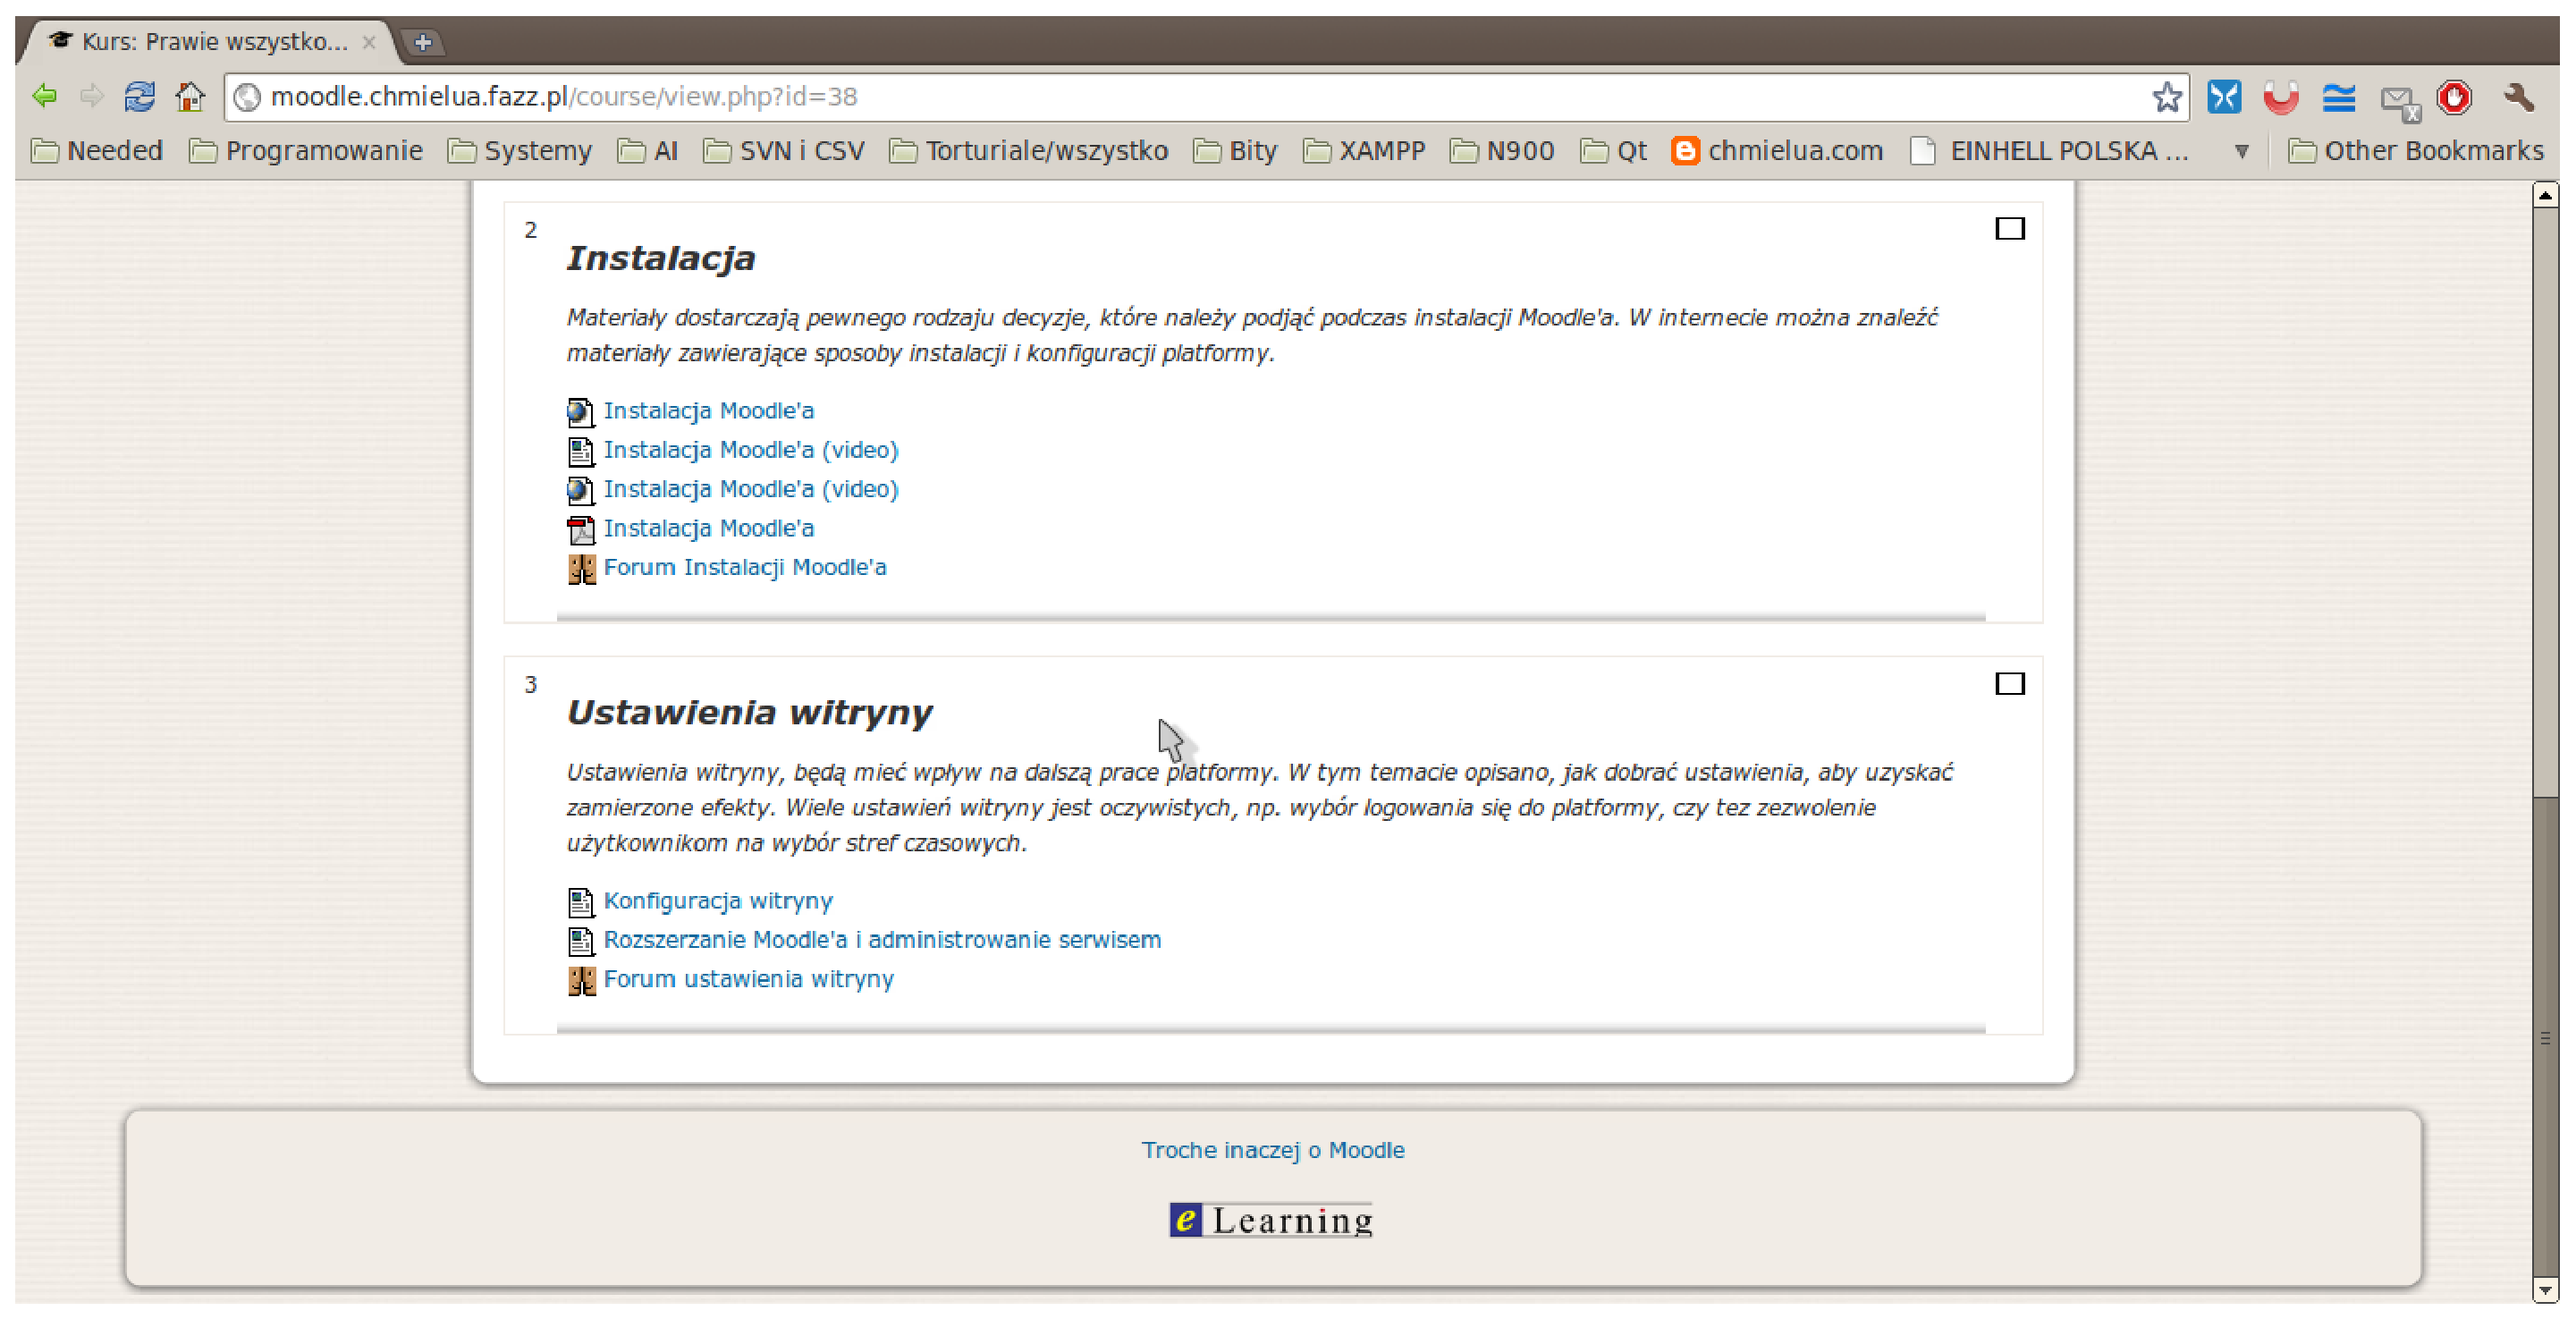
\includegraphics[width=1\textwidth]{projekt_sys//rys//kurs_moodle2.eps}
\end{figure}
Należy wybrać kurs. Przeniesie to nas do strony podzielonej na trzy tematy:
\begin{itemize}
	\item \textit{Wprowadzenie}
	\item \textit{Instalacja}
	\item \textit{Ustawienia witryny}
\end{itemize}
Rys. \ref{rys:kurs_moodle} \ref{rys:kurs_moodle2} pokazują wygląd kursu. Każdy z tematów zawiera materjały dydaktyczne w róznych formach. Na stronie widać że cały kurs posiada forum aktualności i czat. Każdy temat ma swoje osobne forum gdzie mogą być rozstrzygane problemy lub tez można dyskutować na dany temat. \\
\ \\
Administrator platformy posiada dość ciekawy zestaw narzędzi do przeglądania raportów i statystyk rys. \ref{rys:stat} dla danego użytkownika. Dzięki narzędziu GeoIP administrator jest w stanie okreslić skąd pochodziło dane logowanie. Usługa GeoIP identyfikuje pochodzenie adresu IP jak to pokazuje rys. \ref{rys:geoip}. Wynik rozpoznania pokazywany jest z wykorzystaniem narzędzia Google Map.
\begin{figure}[!h]
	\centering
		\caption{Narzędzie GeoIP} \label{rys:geoip}
		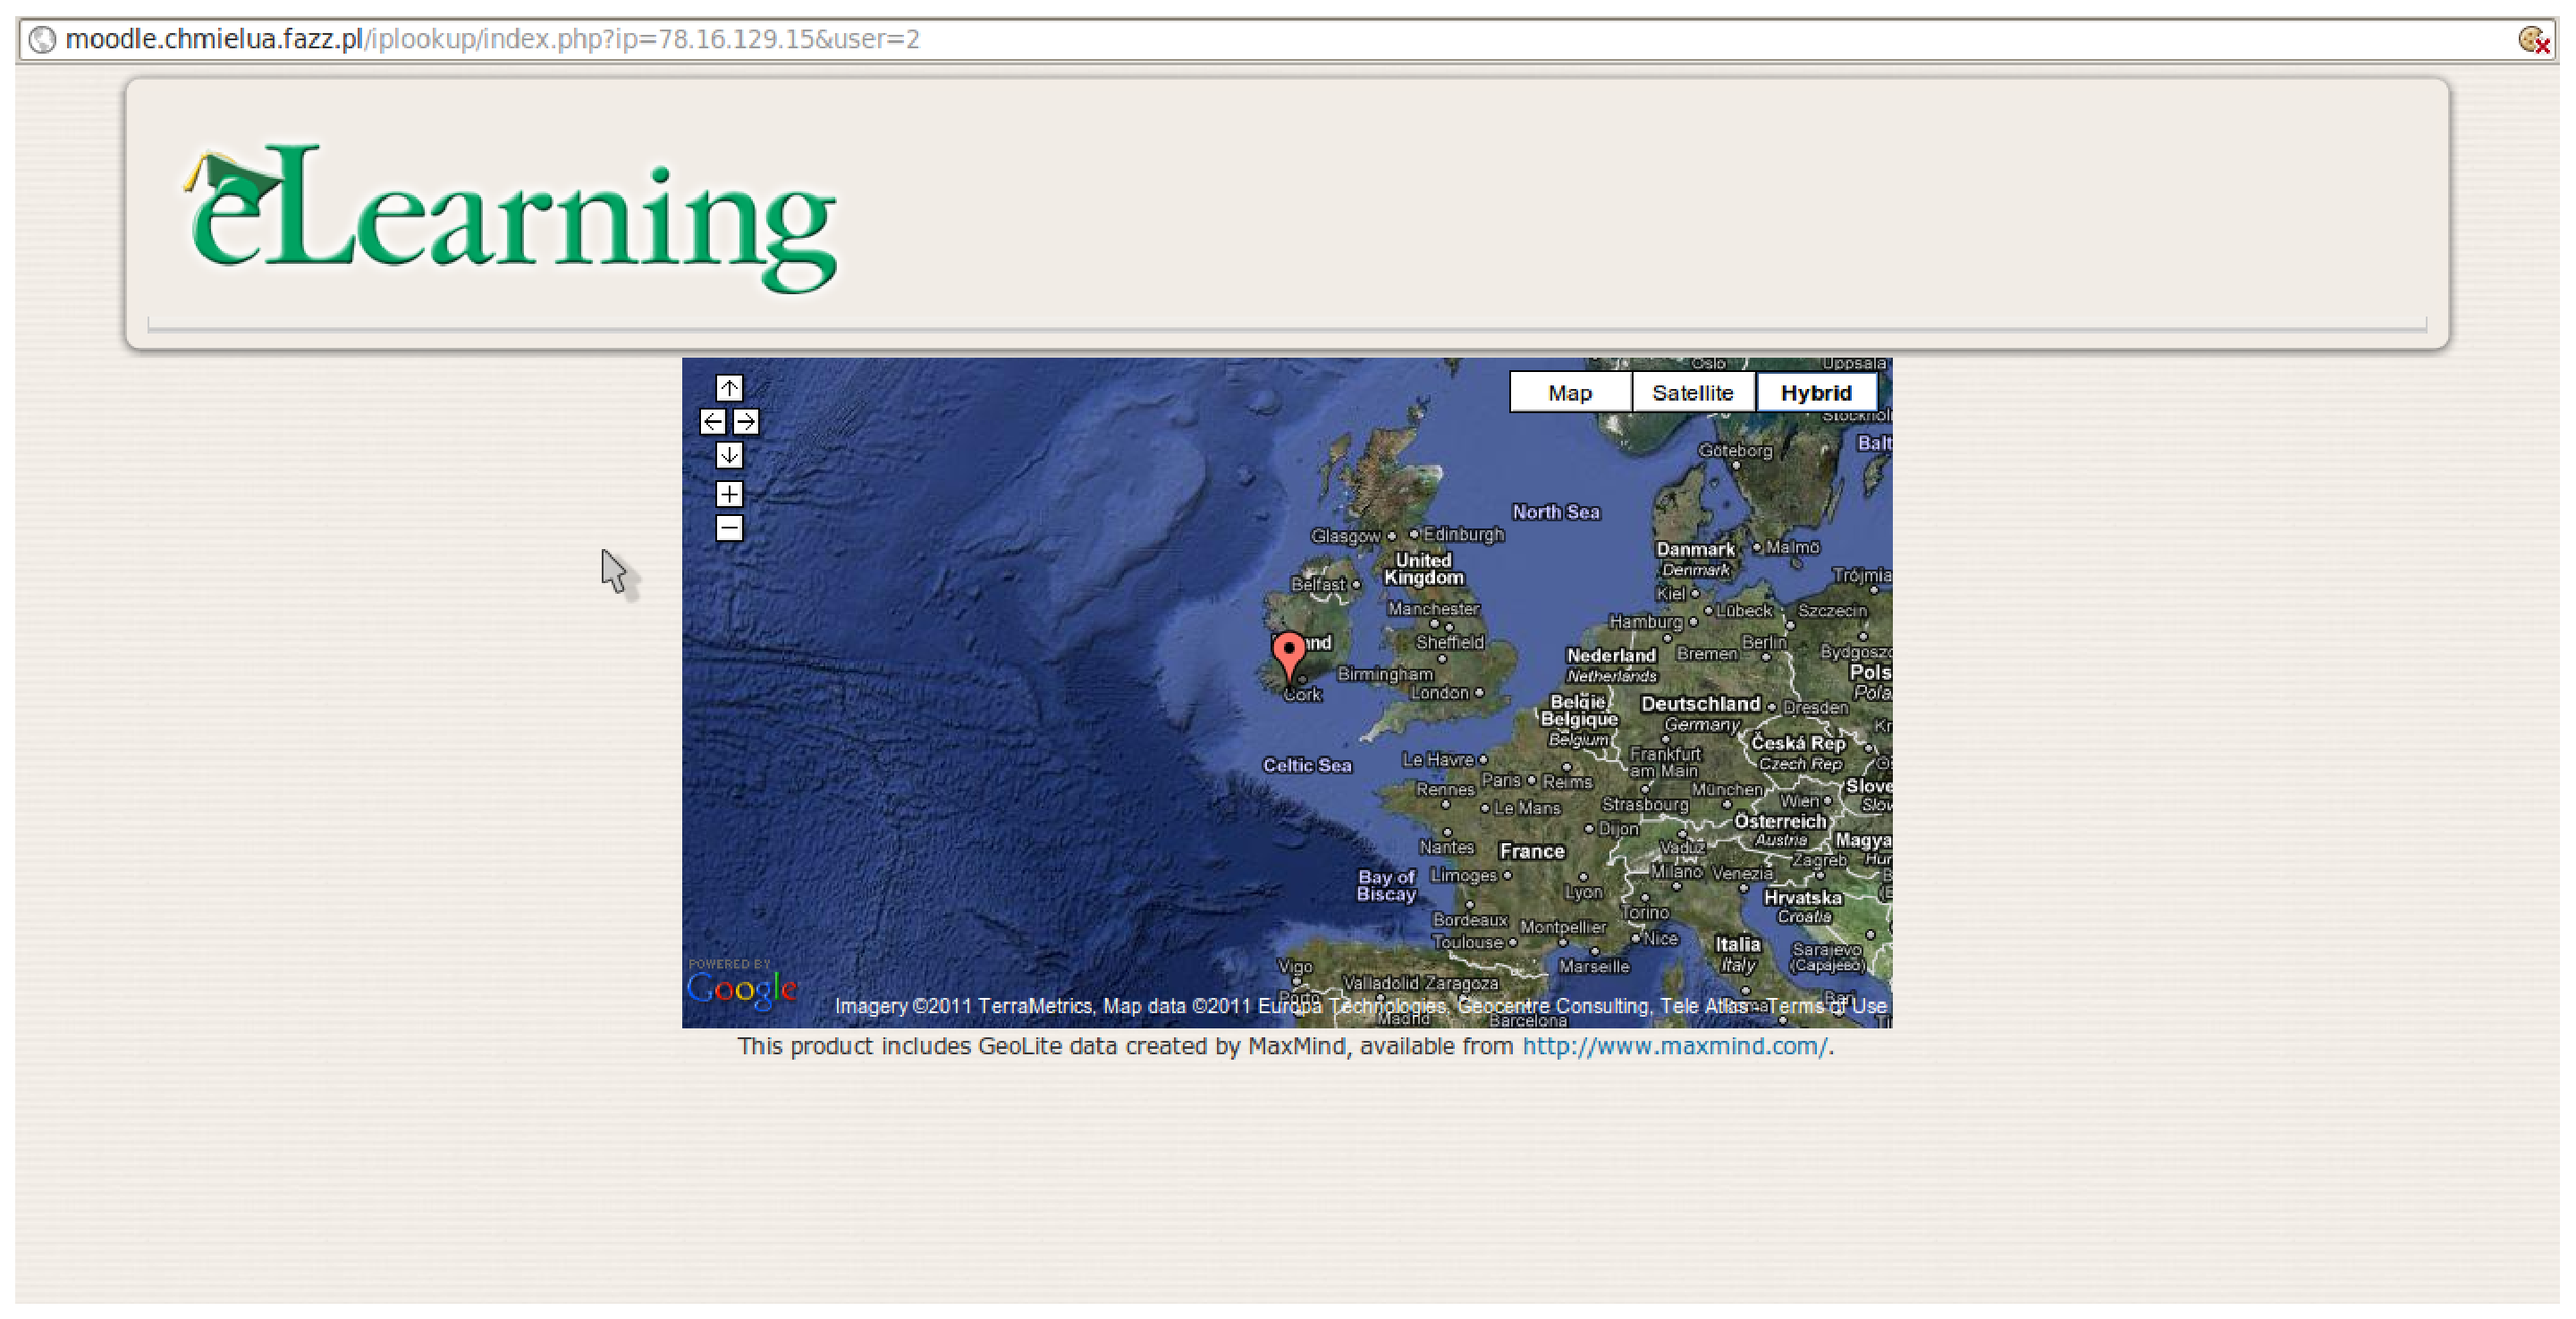
\includegraphics[width=1\textwidth]{projekt_sys//rys//geoip.eps}
\end{figure}
\begin{figure}[!h]
	\centering
		\caption{Przykładowe statystyki} \label{rys:stat}
		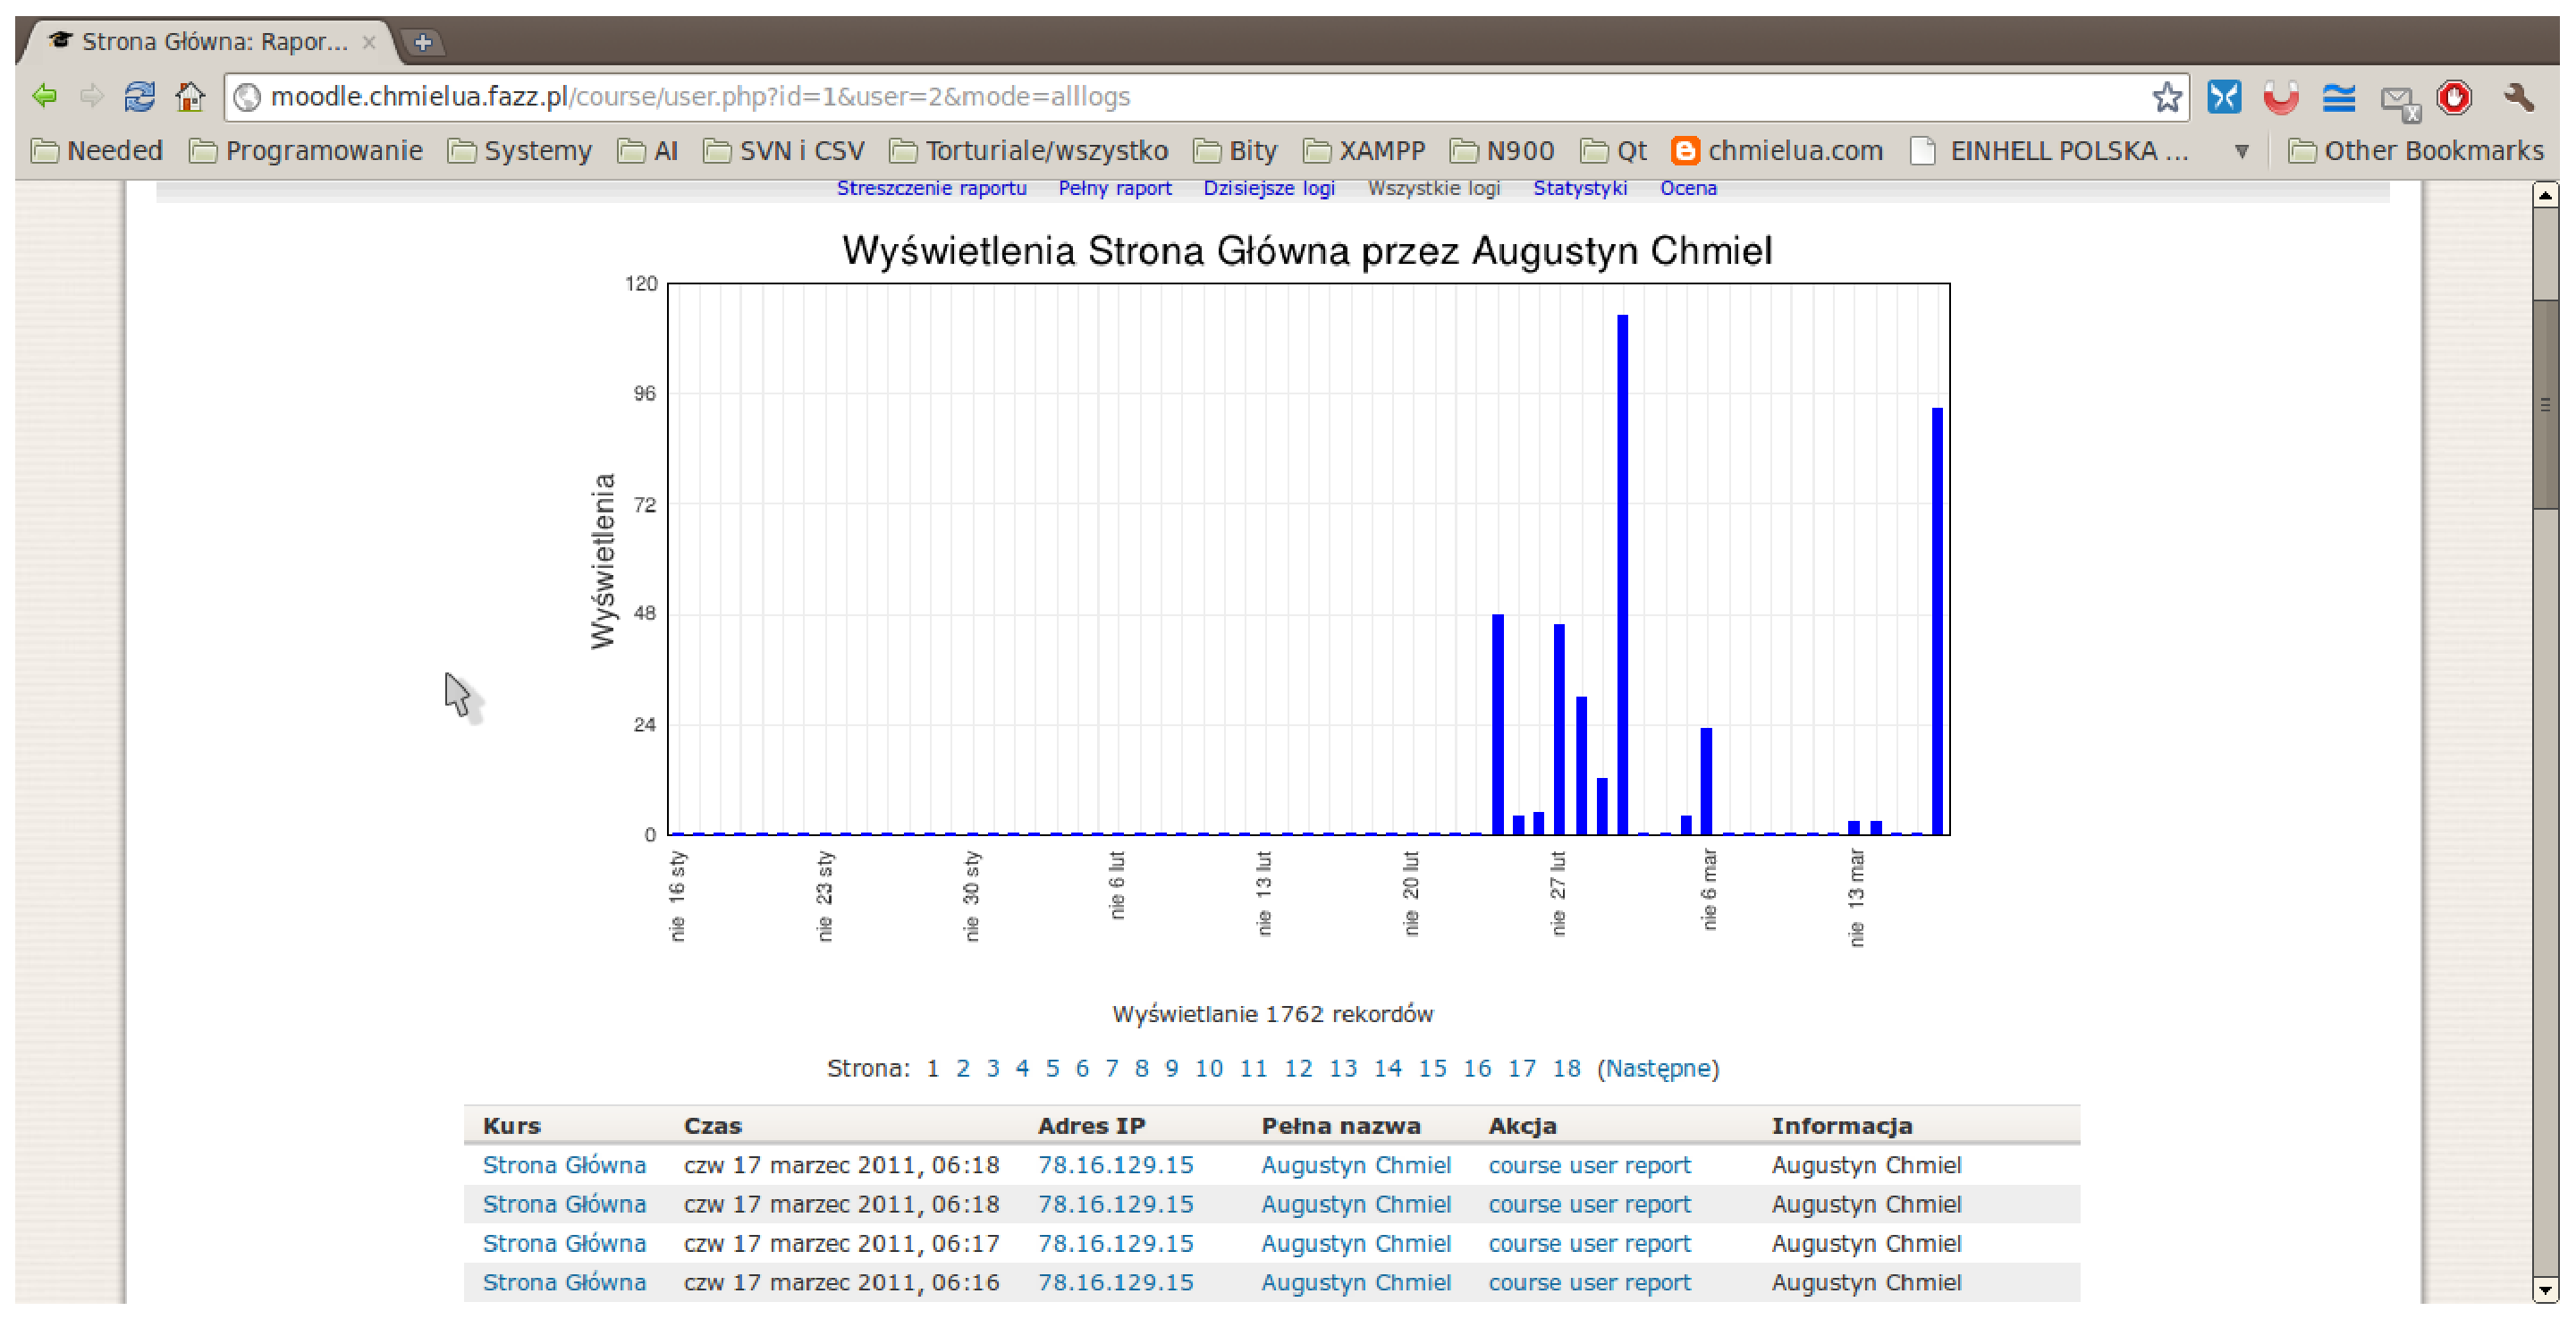
\includegraphics[width=1\textwidth]{projekt_sys//rys//stat.eps}
\end{figure}
\section{Konfiguracja witryny} \label{roz:konfig}
Z menu administracji korzystamy najczęściej podczas tworzenia witryny, w późniejszym czasie korzystamy z niego od czasu do czasu, poprawiając lub też całkiem zmieniając działanie platformy. Aby jednak mieć dostęp do menu administracyjnego trzeba skorzystać z konta administratora. Będąc zalogowanym jako administrator jesteśmy w stanie wpływać na sposób korzystania z witryny przez użytkowników. \\
\ \\
\textbf{Uwierzytelnianie} \\
\ \\
Poprzez uwierzytelnianie rozumiemy sposób logowania się do systemu. I to w jaki sposób system będzie potwierdzał tożsamość logującego się użytkownika. W Moodle'u jest udostępnionych wiele sposobów uwierzytelniania użytkowników. Ich lista znajduje się w rys. \ref{rys:blok_administracji} \textit{Administracja serwisu/Użytkownicy/Uwierzytelnianie/Zarządzaj uwierzytelnianiem} każda z tych opcji jest pokrótce objaśniona po kliknięciu \textit{Ustawienia} rys. \ref{rys:info_uwierz}.
\begin{figure}[!h]
	\centering
		\caption{Blok Administracji serwisu} \label{rys:blok_administracji}
		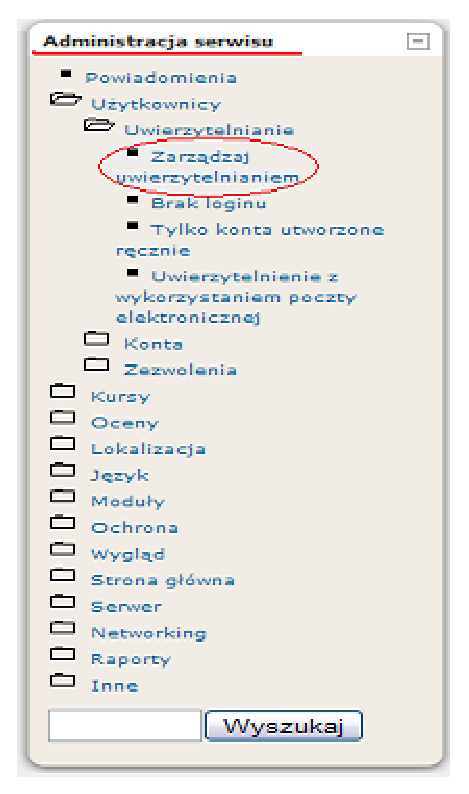
\includegraphics[width = 208px]{projekt_sys//rys//admin.eps}
\end{figure}
\begin{figure}[!h]
	\centering
		\caption{Zarządzanie uwierzytalnianiem} \label{rys:info_uwierz}
		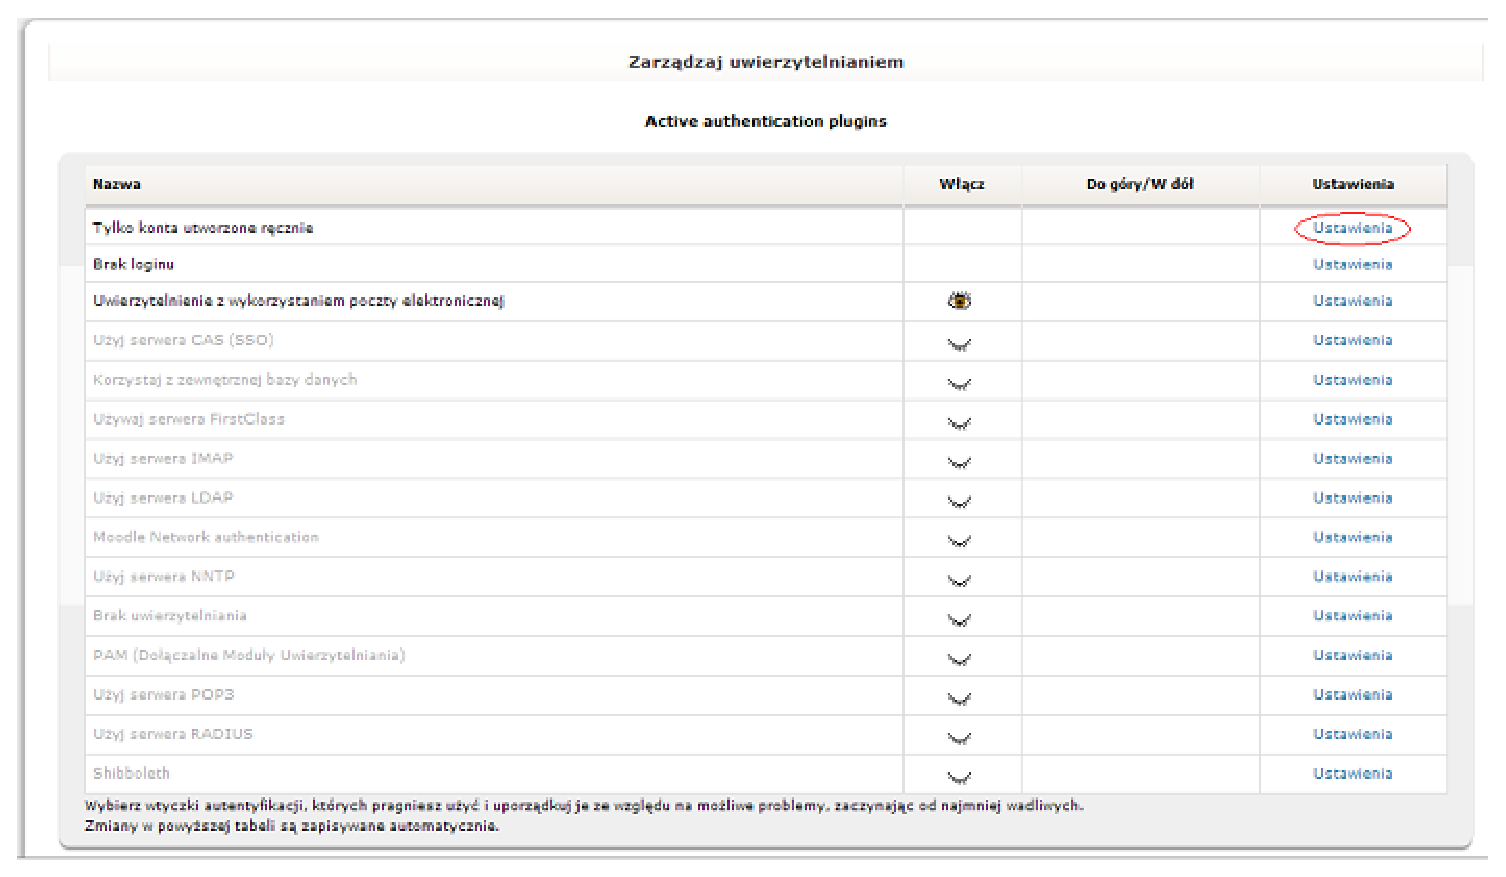
\includegraphics[width=1\textwidth]{projekt_sys//rys//uwierz.eps}
\end{figure}
\textbf{Uwierzytelnianie przy użyciu zewnętrznej bazy danych lub zewnętrznego serwera.}\\
\ \\
W przypadku uwierzytelniania za pomocą zewnętrznej bazy danych hasła można przechowywać na dwa sposoby: \\
\begin{enumerate}
	\item Moodle może tworzyć kopie danych zawartych w zewnętrznej bazie danych, w ustawieniach zewnętrznej bazy danych możemy decydować jak często ma dochodzić do mapowania danych. Teraz gdy użytkownik będzie się logować uwierzytelnianie użytkownika będzie się odbywać z użyciem wewnętrznej bazy danych.
	\item Moodle może również korzystać z zewnętrznej bazy danych przy każdym logowaniu. Przy takim stanie rzeczy Moodle nie przechowuje danych użytkownika w swojej wewnętrznej bazie danych. Nie jest też możliwe zmienianie jakichkolwiek danych przy użyciu platformy. Jeżeli użytkownik będzie chciał edytować jakiekolwiek dane będzie musiał dokonać tych zmian w zewnętrznej bazie danych.
\end{enumerate}
\textbf{Zapisy} \\
\ \\
Zapisy są czymś innym niż uwierzytelnianie. Zapisy określają do jakich kursów użytkownik przynależy, zaś uwierzytelnianie odbywa się podczas logowania do platformy. Tak samo jak przy uwierzytelnianiu, przy zapisach mamy również kilka opcji jakie umożliwiają nam dołączenie do kursu. W menu \textit{Administracja witryny/kursy/zapisy} będziemy mieć listę dostępnych opcji, które po kliknięciu \textit{Modyfikuj} rys. \ref{rys:zapisy} będą pokrótce objaśnione.\\
\begin{figure}[!h]
	\centering
		\caption{Zarządzanie zapisywaniem} \label{rys:zapisy}
		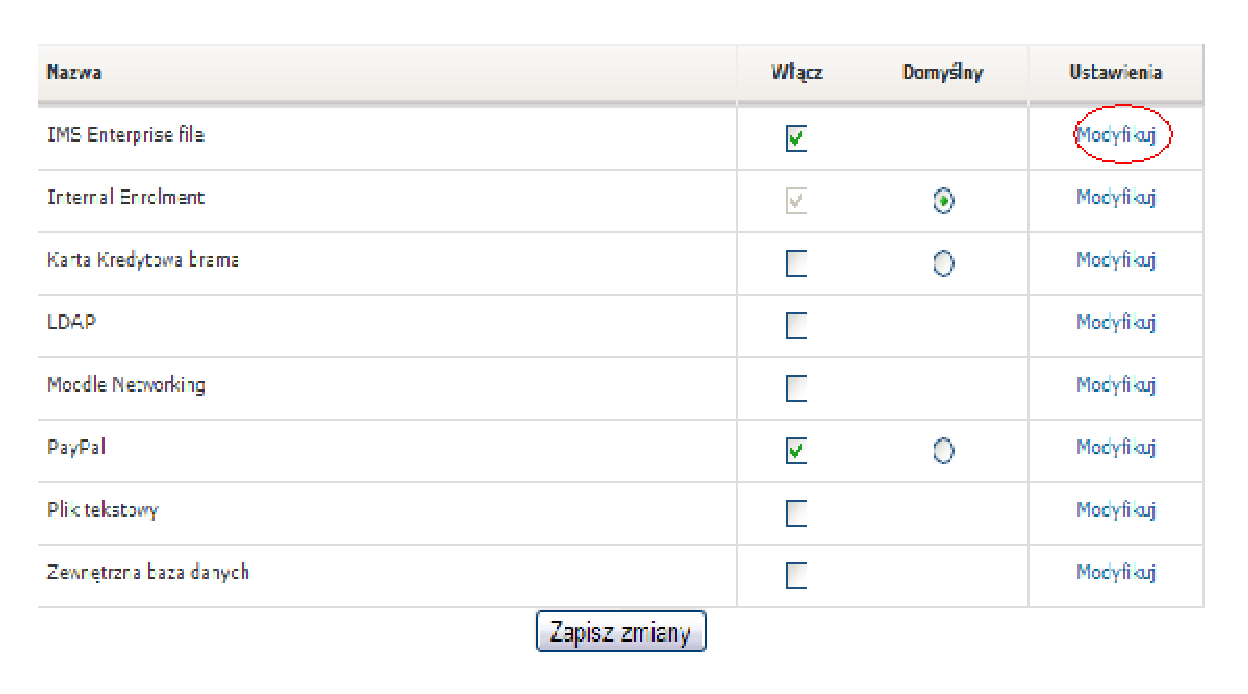
\includegraphics[width=1\textwidth]{projekt_sys//rys//zapisy.eps}
\end{figure}
\textbf{Zapisy wewnętrzne} \\
\ \\
Jest domyślną metodą zapisów. Jeżeli pozostawimy ten rodzaj zapisu, będziemy mieli możliwość zapisu ucznia, poprzez Administratora lub Nauczyciela. Innym rozwiązaniem jest opcja klucz zapisów. Jak się można domyśleć aby móc się zapisać na kurs trzeba będzie posiadać klucz.\\
\ \\
\textbf{Plik tekstowy} \\
\ \\
W przypadku zapisu większej ilości uczniów istnieje możliwość podania listy uczniów poprzez plik tekstowy. Aby móc przeprowadzić zapis poprzez plik tekstowy trzeba utworzyć plik w odpowiednim formacie. \\
\ \\
\textit{opcja, rola, identyfikator użytkownika, identyfikator kursu}\\
np.\\
\textit{add, student, 001, MOODLE01} \\
\ \\
W pliku wpisujemy skrócone nazwy ról "student" gdzie nazwa roli pisana jest wielką literą \textit{Student}. Przykład dla pliku powyżej określa nam że użytkownik o numerze \textit{001} zostanie dodany w roli ucznia do kursu o identyfikatorze \textit{MOODLE01}.\\
\begin{itemize}
	\item \textit{operacja}~-~podajemy tutaj nazwę operacji która ma być wykonana, np. \textit{add, del}
	\item \textit{rola}~-~podajemy nazwę roli jaka użytkownik będzie pełnił w kursie, \textit{student, teacher, admin}
	\item \textit{identyfikator użytkownika}~-~inaczej numer id, pole to znajduje się w profilu każdego użytkownika, aby moc skorzystać z funkcji pliku pole to musi mieć nadany identyfikator.
	\item \textit{identyfikator kursu}~-~jest to unikalny identyfikator danego kursu, może być nadawany np. podczas tworzenia kursu.
\end{itemize}
\begin{figure}[!h]
	\centering
		\caption{Numer ID użytkownika} \label{rys:nr_id}
		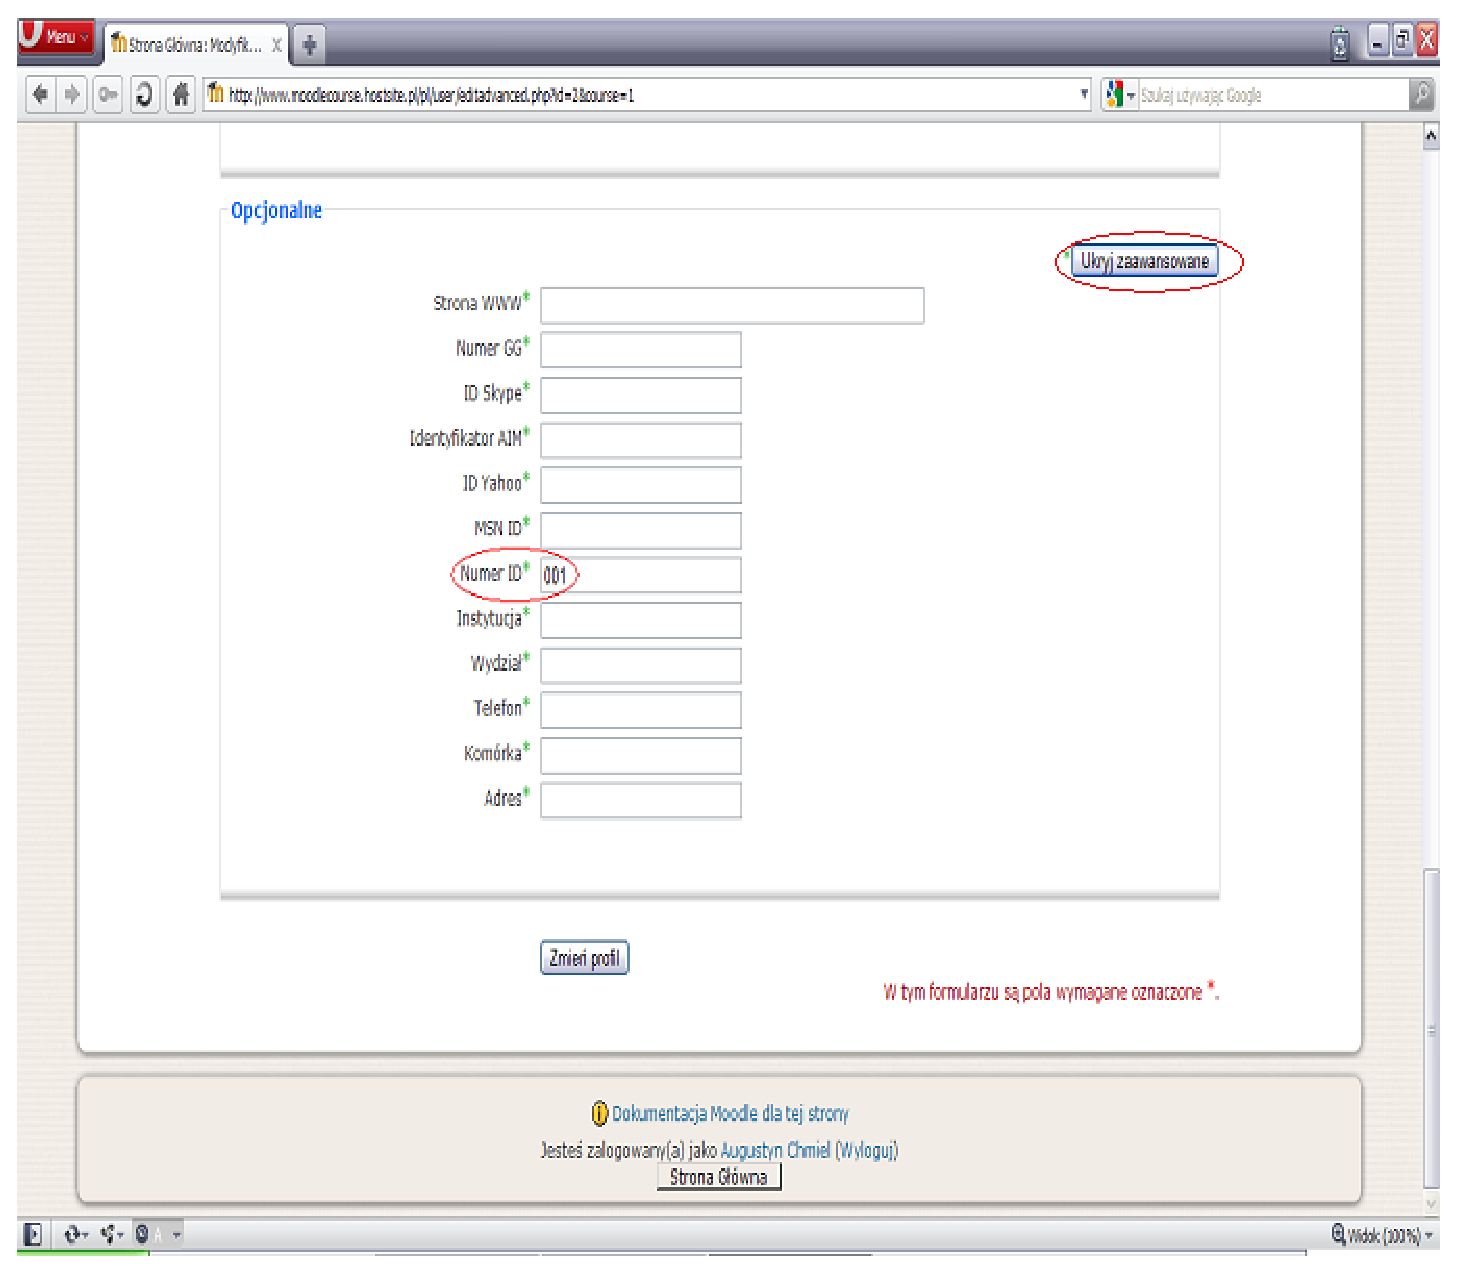
\includegraphics[width=1\textwidth]{projekt_sys//rys//nr_id.eps}
\end{figure}
Identyfikator ucznia jest wymagany przy metodzie zapisów za pomocą pliku tekstowego. W bazie danych znajduje on się w tabeli mdl\_user w kolumnie idnumber. Najszybszym sposobem wypelnienia tych pól jest zgłoszenie takiego zadania administratorowi który odpowiednia komenda SQL wypełni wszystkie pola. Na przykład coś takiego:
\begin{verbatim}
use moodle;
delimiter $

CREATE PROCEDURE id_number(id_max INT)
	BEGIN
		set @id_start = id_max - (id_max - 1);
		WHILE @id_start < id_max do
			UPDATE mdl_user SET idnumber = @id_start
                                        WHERE id = (@id_start + 1);
			set @id_start = @id_start + 1;
		END WHILE;
        END$
delimiter ;

CALL id_number((SELECT max(id) from mdl_user));
\end{verbatim}
Przydatna informacją też jest fakt że pole to jest typu VARCHAR(255) - czyli łańcuchem znaków o zmiennej długości, max 255 znaków. Również szybszym sposobem niż edycja każdego użytkownika z osobna w Moodle'u będzie skorzystanie z panelu phpMyAdmin, gdzie można w trochę szybszy sposób wyklinać wszystko i nanieś poprawki ręcznie rys. \ref{rys:baza_users},
\begin{figure}[!h]
	\centering
		\caption{Tabela użytkowników \textit{mdl\_users}} \label{rys:baza_users}
		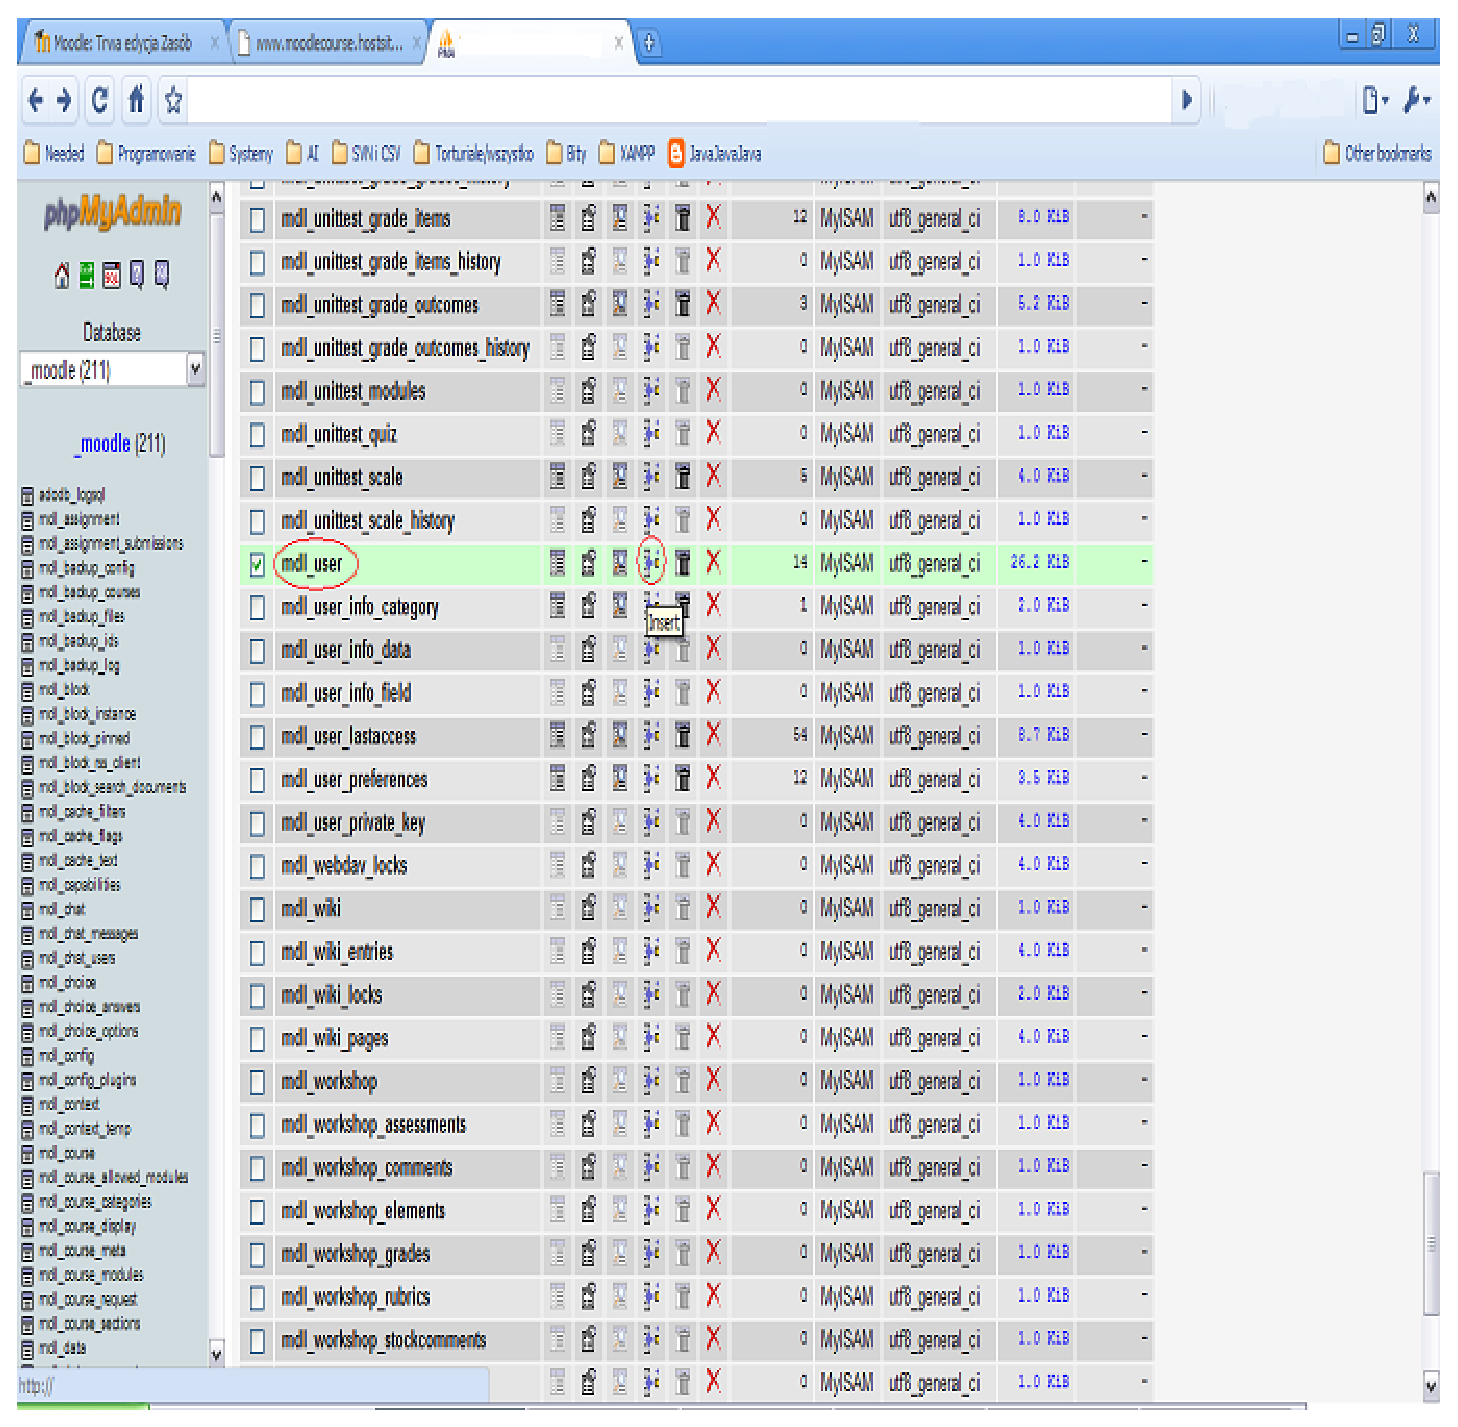
\includegraphics[width=1\textwidth]{projekt_sys//rys//baza_users.eps}
\end{figure}
\ref{rys:insert},
\begin{figure}[!h]
	\centering
		\caption{Dodanie użytkownika do \textit{mdl\_users} } \label{rys:insert}
		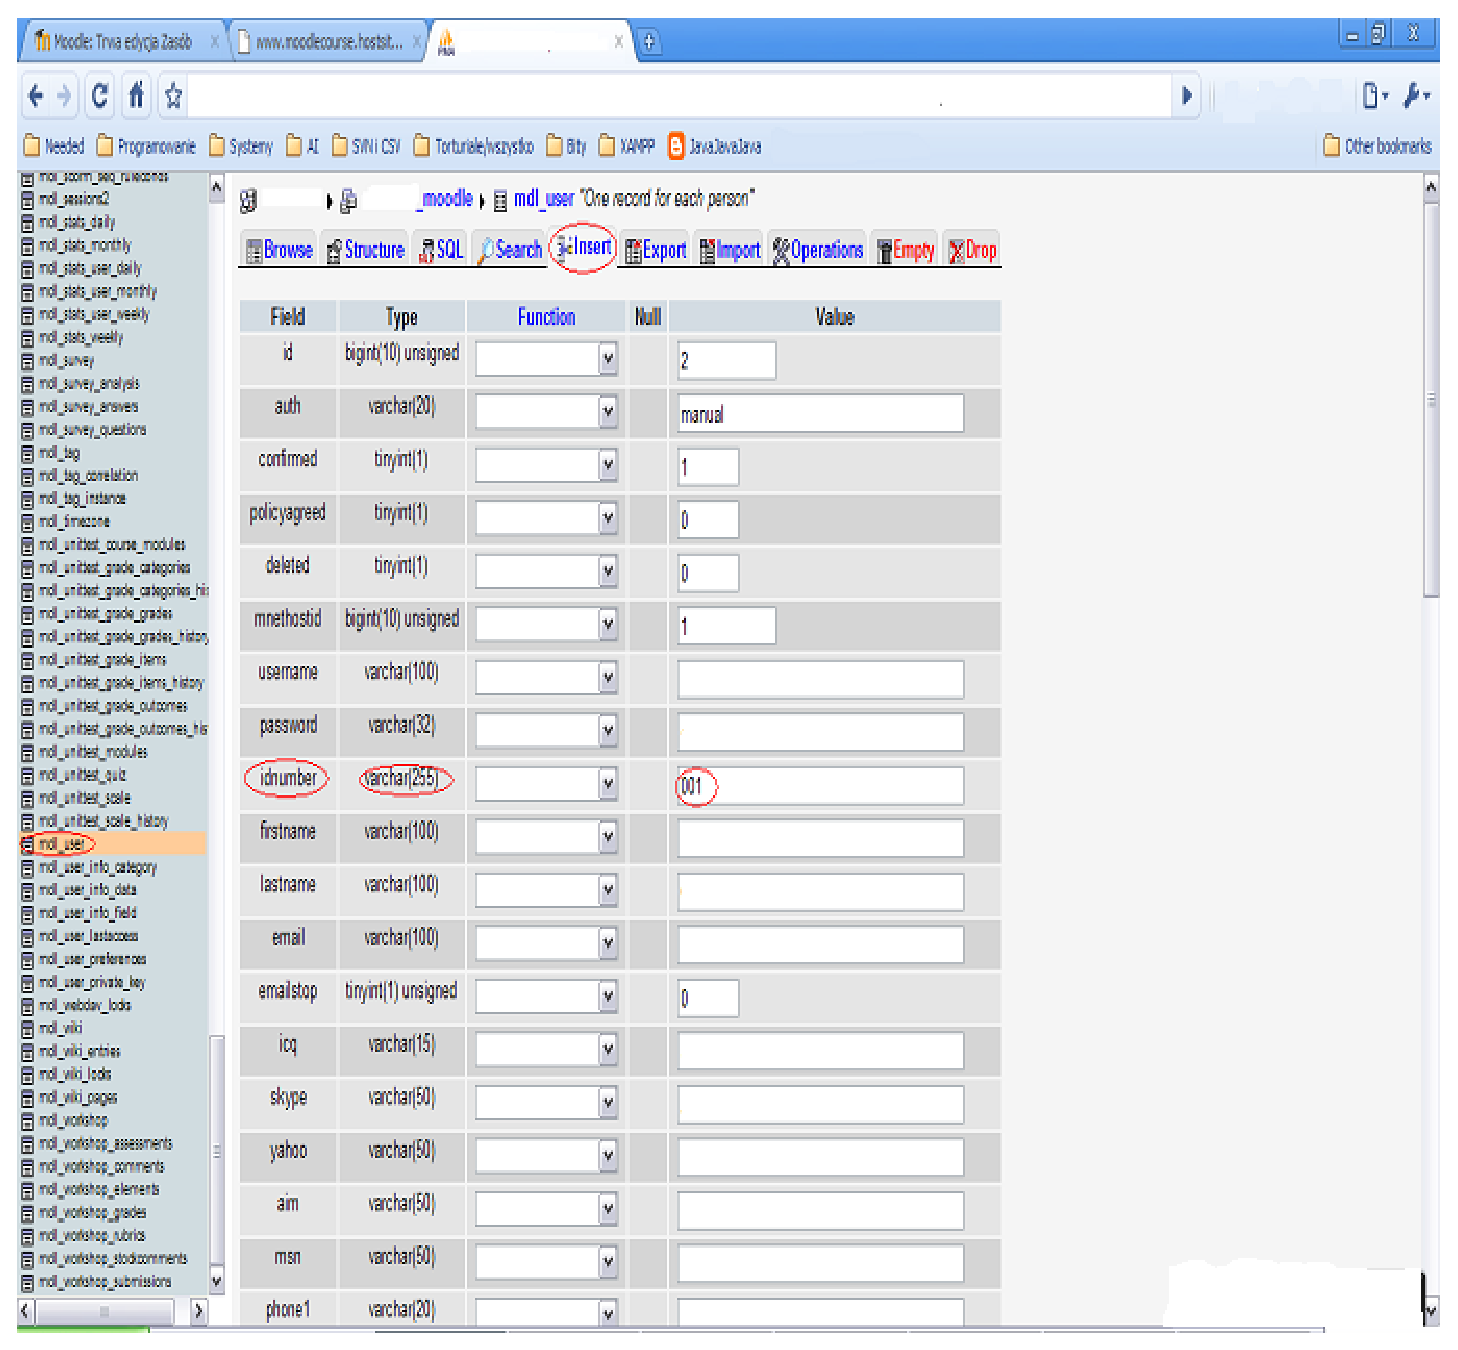
\includegraphics[width=1\textwidth]{projekt_sys//rys//insert.eps}
\end{figure}
\ref{rys:tab_user}.
\begin{figure}[!h]
	\centering
		\caption{Tabela \textit{mdl\_users}} \label{rys:tab_user}
		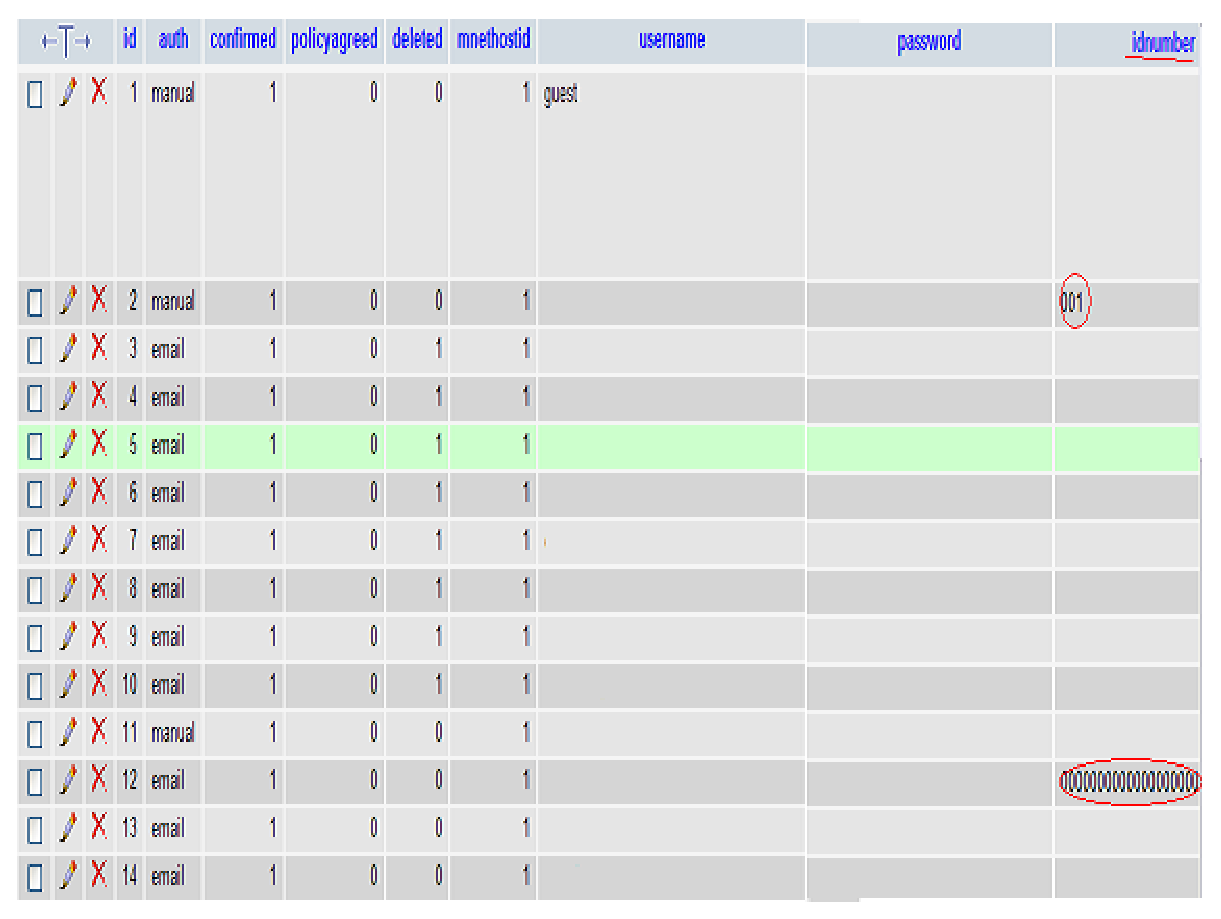
\includegraphics[width=1\textwidth]{projekt_sys//rys//tab_user.eps}
\end{figure}
A tak wygląda nasza baza po wykonaniu bardzo prostej procedury, mała rzecz, a cieszy ;) rys. \ref{rys:baza_id_users}.
\begin{figure}[!h]
	\centering
		\caption[Tabela \textit{mdl\_users} po wykonaniu procedury]{Tabela użytkowników \textit{mdl\_users} po wykonaniu procedury} \label{rys:baza_id_users}
		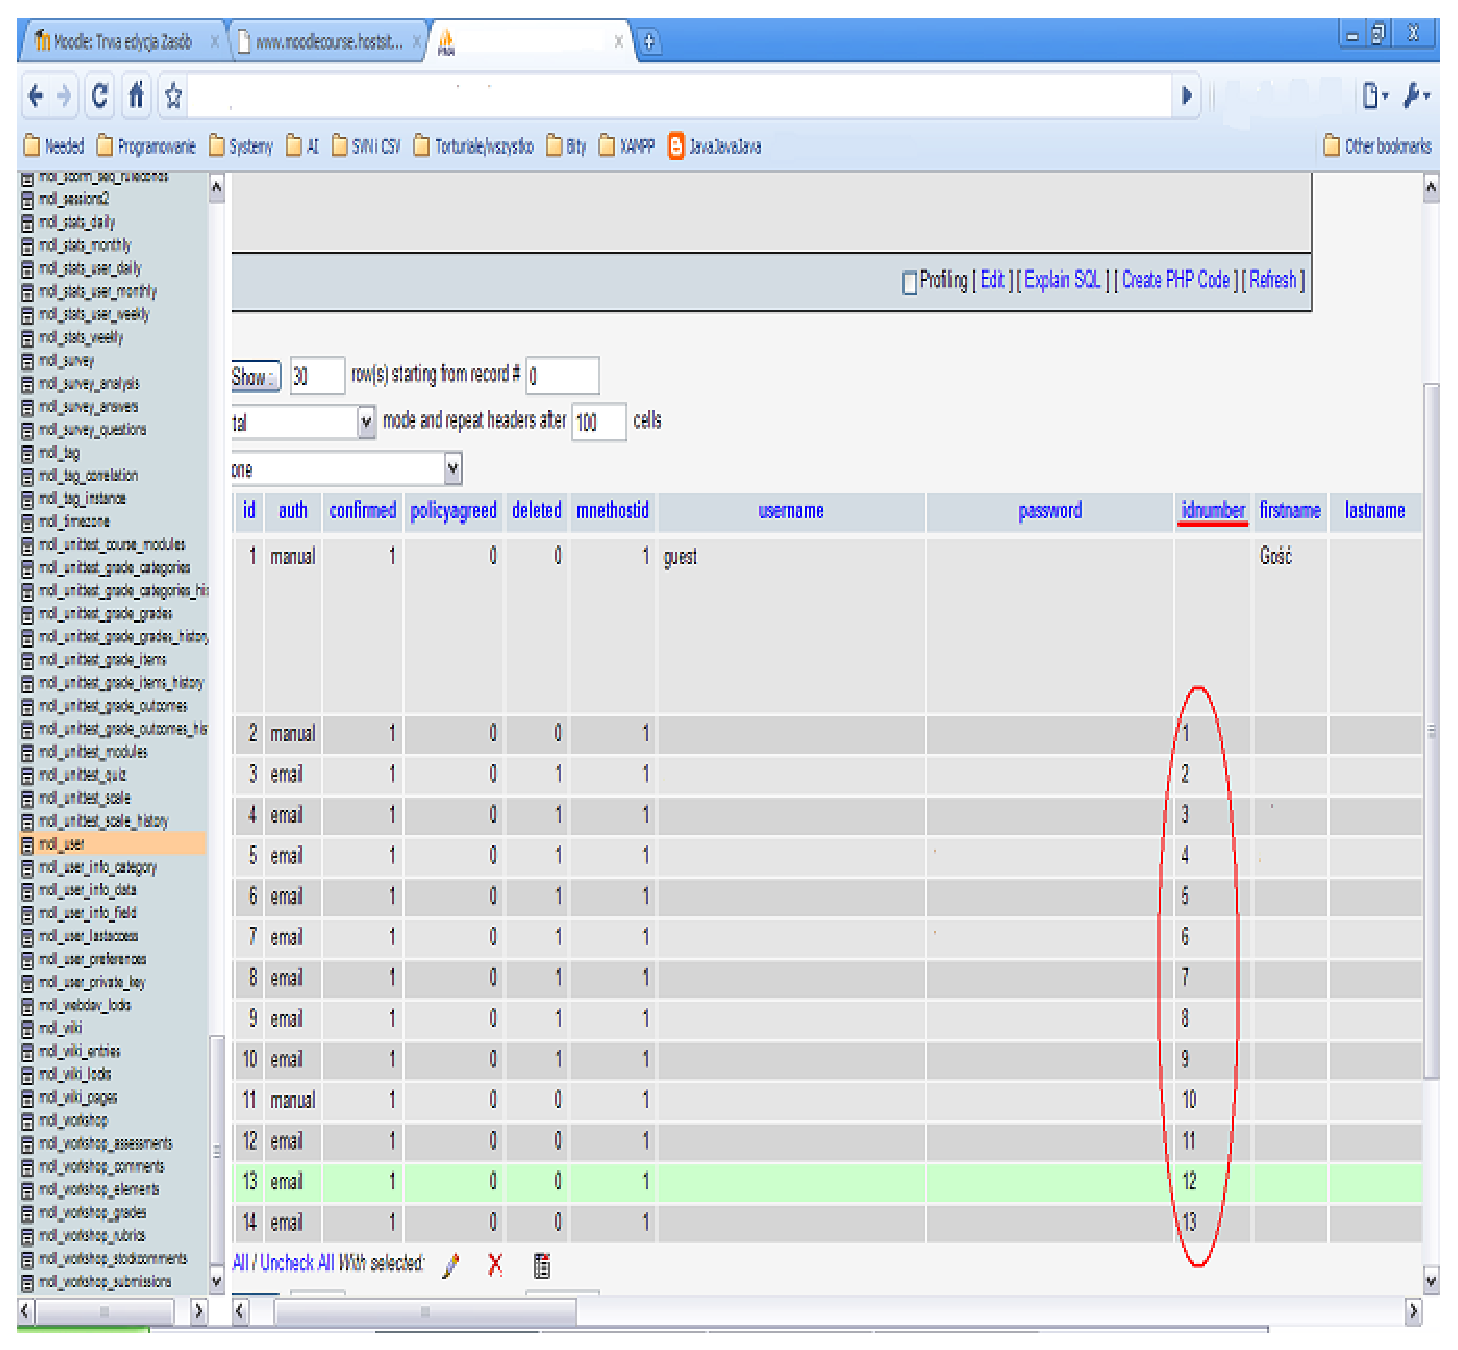
\includegraphics[width=1\textwidth]{projekt_sys//rys//procedura.eps}
\end{figure}
To jest jeden z przykładów jakiegoś tam rozwiązania można również zastosować jakiś wyzwalacz, który automatycznie po dodaniu użytkownika do tabeli nada mu jego \textit{idnumber}. Po prostu pokazuje tutaj ze można znacznie ułatwić sobie życie takimi pomysłami administrując w ten sposób platformę. \\
\ \\
Identyfikator kursu analogicznie jak to było z identyfikatorem użytkownika jest polem opcjonalnym. W bazie danych Moodle'a identyfikator kursu można znaleźć w tabeli \textit{mdl\_course} i również w kolumnie \textit{idnumber}. Tyle że w tym przypadku mamy pole typu \textit{VARCHAR(100)} czyli łańcuch o zmiennej długości, o maksymalnym zakresie 100 znaków. \\
\ \\
\textbf{Rola} \\
\ \\
Role określają nam status użytkownika, czyli mówią nam co dany użytkownik może a czego nie może. Ważnym punktem tutaj jest powiedzenie że użytkownik może mieć określoną role dla witryny, jak i również dla danego kursu i nie musi ona być taka sama jaka jest zdefiniowana dla witryny. Aby sprawdzić wszystkie domyślnie zdefiniowane role, oraz poznać ich skrócone nazwy, należy przejść do Administracja witryny/Użytkownicy/Uprawnienia/Definicje ról po wyborze roli z listy dostaniemy dokładniejsze informacje na temat roli.\\
\ \\
\textbf{Format IMS Enterprise} \\
\ \\
Jest to plik XML, który jest zgodny ze standardami okreslonymi przez \textbf{IMS Global Learning Consortium}. Pliki tego formatu maja bardzo wiele zastosowań z których głównie korzystają instytucje z systemami zarządzania zasobami ludzkimi, więcej na ten temat można znaleźć tu.\\
\ \\
\textbf{LDAP}\\
\ \\
LDAP może być wykorzystywany do zapisów jak i do uwierzytelniania, korzystając z LDAP przy zapisach, nie zmusza to nas do korzystania z niego przy uwierzytelnianiu i na odwrót.\\
\ \\
\textbf{Zewnętrzna baza danych} \\
\ \\
Moodle do obecnej wersji 1.9 nie wspiera zewnętrznej bazy danych, czyli wszystkie zmiany danych jakich trzeba dokonać w zewnętrznej bazie danych muszą być dokonywane przez inny program. Podczas korzystania z zewnętrznej bazy danych przy zapisach na kursy, możemy również korzystać z bazy wewnętrznej w Moodle'u. W ustawieniach zewnętrznej bazy danych trzeba zdefiniować pole po którym dane z wewnętrznej bazy danych będą kojarzone z bazą zewnętrzną. Mianowicie do pola o nazwie \textit{enrol\_localcoursefield} należy podać nazwę kolumny z tabeli \textit{mdl\_course}. Nazwa kolumny która nas interesuje to znów nasze \textit{idnumber} i tak samo postępujemy z następnym polem o nazwie \textit{enrol\_localuserfield} znów podajemy \textit{idnumber}.\\
\ \\
\textbf{Wybór języka}\\
\ \\
Przy wyborze języka dobrze jest się zastanowić już na samym początku tworzenia naszej platformy. Mianowicie instalacja Moodle'e zawiera wiele pakietów językowych, które służą do tłumaczenia interfejsu a nie zasobów kursu. Może się również zdarzyć że jakaś część interfejsu nie została przetłumaczona, wówczas Moodle używa domyślnie wersji językowej angielskiej. W celu dokładniejszego przetłumaczenia interfejsu można się pokusić o pogrzebanie w plikach znajdujących się w katalogu \textit{/moodledata/lang/} i tak np. dla jeżyka polskiego następnym katalogiem będzie \textit{/pl\_utf8/}. Moodle może nam podać dokładną liczbę brakujących tłumaczeń. W tym celu należy się udać \textit{Administracja/Język/Edycja języka}. Platforma posiada tłumaczenia, ale tylko i wyłącznie samych interfejsów. W celu uzyskania pełnego tłumaczenia wraz z zawartością kursów, mamy dostępne następujące opcje: \\
Utworzenie dokumentów dla danego kursu w rożnych językach, co moim zdaniem jest jakiś rozwiązaniem, ale daje dość brzydki bałagan na stronie kursu czy też w kursach. \\
\ \\
Drugą opcją jest utworzenie różnych kursów w rożnych językach.\\
\ \\
Trzecią możliwością jest utworzenie odrębnej platformy Moodle'a dla każdego języka np. \textit{http://www.moodlecourse.pl/pl/} dla języka polskiego i \textit{http://www.moodlecourse.pl/en/} dla języka angielskiego. Na stronie głównej uczniowie wybierają język i są automatycznie przekierowywani do odpowiedniej instalacji Moodle'a. Więc widzimy że chcąc udostępniać platformę w różnych językach dobrze jest rozważyć taką sytuacje przed instalacją Moodle'a. \\
\  \\
Ostatnią możliwością jest zastosowanie filtrów. Rodzaje filtrów i ich ustawienia znajdziemy tu: \textit{Administracja/Moduły/Filtry/Filtruj} ustawienia następnie należy włączyć filtr o nazwie treść wielojęzyczna, aby nasz filt prawidłowo zadziałał należy umieścić tekst w znacznikach \textit{<spam>} w następujący sposób:\\
\begin{verbatim}
<span lang = "en">English Course</span>
<span lang = "pl">Polski kurs</span>   
\end{verbatim}
\section{Plan tworzenia witryny nauczania} \label{roz:plan}
W tym podrozdziale przedstawie liste zadan jakie należy wykonać, aby utworzyć witryne nauczania z wykorzystaniem platformy Moodle (źródło: \cite{tworzenie_serwisow}):
\begin{enumerate}
	\item Planowanie kursu.
	\begin{description}
		\item[a)] Określenie celów nauczania~-~należy określić jąką wiedze mają posiąść użytkownicy w trakcie kursu.
		\item[b)] Zbieranie materiałów do kursu. 
		\item[c)] Zastanowienie się nad ideą konstrukcjonizmu społecznego. Zaplanowanie sposobu nauki online pozwalającego na eksplorację i instalację.
	\end{description}
	\item Instalacja i konfiguracja Moodle'a.
	\begin{description}
		\item[a)] Instalujemy Moodle'a...
		\begin{itemize}
			\item Otrzymanie uprawnień na serwerze, który spełnia wymagania Moodle'a.
			\item Utworzenie poddomen i/lub katalogów potrzebnych do instalacji Moodle'a i do przechowywania jego danych.
			\item Pobranie i rozpakowanie Moodle'a oraz przesłanie go na serwer.
			\item Utworzenie katalogu danych Moodle'a.
			\item Utworzenie bazy danych Moodle'a.
			\item Ustawienie zadań corna.
			\item Aktywacja instalacji.
		\end{itemize}
		\item[b)] Jeżeli administrujemy witrynę lub tworzymy kursy...
		\begin{itemize}
			\item Konfiguracja zmiennych dla całej witryny.
			\item Konfiguracja ustawien dla całej witryny.
			\item Konfiguracja uwierzytelniania i kopii zapasowych.
		\end{itemize}
	\end{description}
	\item Tworzenie struktury witryny nauczania.
	\begin{description}
		\item[a)] Tworzenie i porządkowanie kategorii kursów.
		\item[b)] Tworzenie kursów.
		\begin{itemize}
			\item Konfiguracja ustawień kursu.
			\item Porządkowanie kursów w kategoriach.
			\item Przypisywanie ról nauczycielom.
		\end{itemize}
		\item[c)] Wybieranie bloków do wyświetlaniaw całej witrynie.
		\item[d)] Wybieranie bloków do wyświetlania w poszczególnych kursach.
	\end{description}
	\item Dodawanie podstawowego materiału do kursów.
		\begin{description}
			\item[a)] Dodawanie materiałów do czytania: stron tekstowych i internetowych.
			\item[b)] Dodawanie odnośników do innych witryn.
			\item[c)] Tworzenie katalogów plików i przesyłanie plików do nich.
			\item[d)] Porządkowanie materiału w tematy lub tygodnie.
			\item[e)] Dodawanie etykiet.
			\item[f)] Dodawanie bloku \textit{Activities (elementy interaktywne)}, jeżeli jest potrzebny.
		\end{description}
	\item Tworzenie elementów interaktywnych.
		\begin{description}
			\item[a)] Dodawanie zadań.
			\item[b)] Dodawanie głosowań.
			\item[c)] Dodawanie dzienników uczniów.
			\item[d)] Tworzenie lekcji
			\begin{itemize}
				\item Zaplanowanie przebiegu lekcji.
				\item Określenie kryteriów oeniania.
				\item Dodawanie materiałów do lekcji.
				\item Dodawanie pytań i przejść pomiędzy nimi.
			\end{itemize}
			\item[e)] Tworzenie quizów.
			\begin{itemize}
				\item Tworzenie kategorii pytań.
				\item Tworzenie pytań.
				\item Wybieranie pytań do quizów.
			\end{itemize}
		\end{description}
	\item Tworzenie elementów społecznościowych.
	\begin{description}
		\item[a)] Dodawanie czatów, opcjonalnie można je ukryć do czasu zaplanowanego czasu spotkania.
		\item[b)] Jeżeli czaty są zaplanowane, dodanie bloków \textit{Calendar (kalendarz)} i \textit{Upcoming Events (nadchodzące wydarzenia)}.
		\item[c)] Dodawanie forów dla uczniów do witryny i kursów.
		\item[d)] Dodawanie forów dla nauczycieli.
		\item[e)] Dodawanie ukrytych forów, w celu przesyłania masowych e-maili.
		\item[f)] Dodawanie lokalnych i globalnych słowników pojęć.
		\item[g)] Dodawanie stron wiki i konfigurowaniedostępu do nich.
		\item[h)] Dodawanie warsztatów.
			\begin{itemize}
				\item Jakie będzie zadanie dla każdego z uczniów ?
				\item Kto będzie mógł zobaczyć przesyłane zadania ?
				\item W jaki sposób zadania będą oceniane ?
				\item Kiedy uczniowie będą mogli przesłać swoje zadania ?
			\end{itemize} 
	\end{description}
	\item Tworzenie strony powitalnej dla nowych i zarejestrowanych w systemie użytkowników.
	\begin{description}
		\item[a)] Decydowanie o pozwoleniu na dostęp przez konto gościa lub anonimowy dostęp do całej witryny lub jej części.
		\item[b)] Wybór strony powitalnej dla nowych użytkowników~-~strona logowania lub strona główna.
		\item[c)] Modyfikacje wyglądu i zachowania strony logowania.
		\item[d)] Dodawanie materiałów do strony głównej. Tworzenie kursu, którym jest strona główna.
		\item[e)] Modyfikacje wyglądu witryny.
	\end{description}
	\item Wykorzystanie narzędzi nauczycieli w celu zarządzania i administracji kursami.
	\begin{description}
		\item[a)] Tworzenie własnych skal oceniania.
		\item[b)] Tworzenie forów dla nauczycieli.
		\item[c)] Interpretacja logów dostępu.
		\item[d)] Wyświetlanie i pobieranie ocen uczniów.
	\end{description}
	\item Rozszerzanie możliwości Moodle'a~-~dodatkowe moduły.
	\begin{description}
		\item[a)] Instalacja i integracja dodatkowych modułów.
		\item[b)] Testowanie dodatkowych modułów.
		\item[c)] Tworzenie kopii zapasowych modułów i/lub witryny.
		\item[d)] Wykorzystanie modułu PayPal w celu tworzenia płatnych kursów i witryn.
	\end{description}
\end{enumerate}

\section{Schematy blokowe} \label{roz:schematy}
\begin{figure}[!h]
	\centering
		\caption[Instalacja Moodle'a]{Schemat blokowy Instalacji Moodle'a} \label{rys:instalacja}
		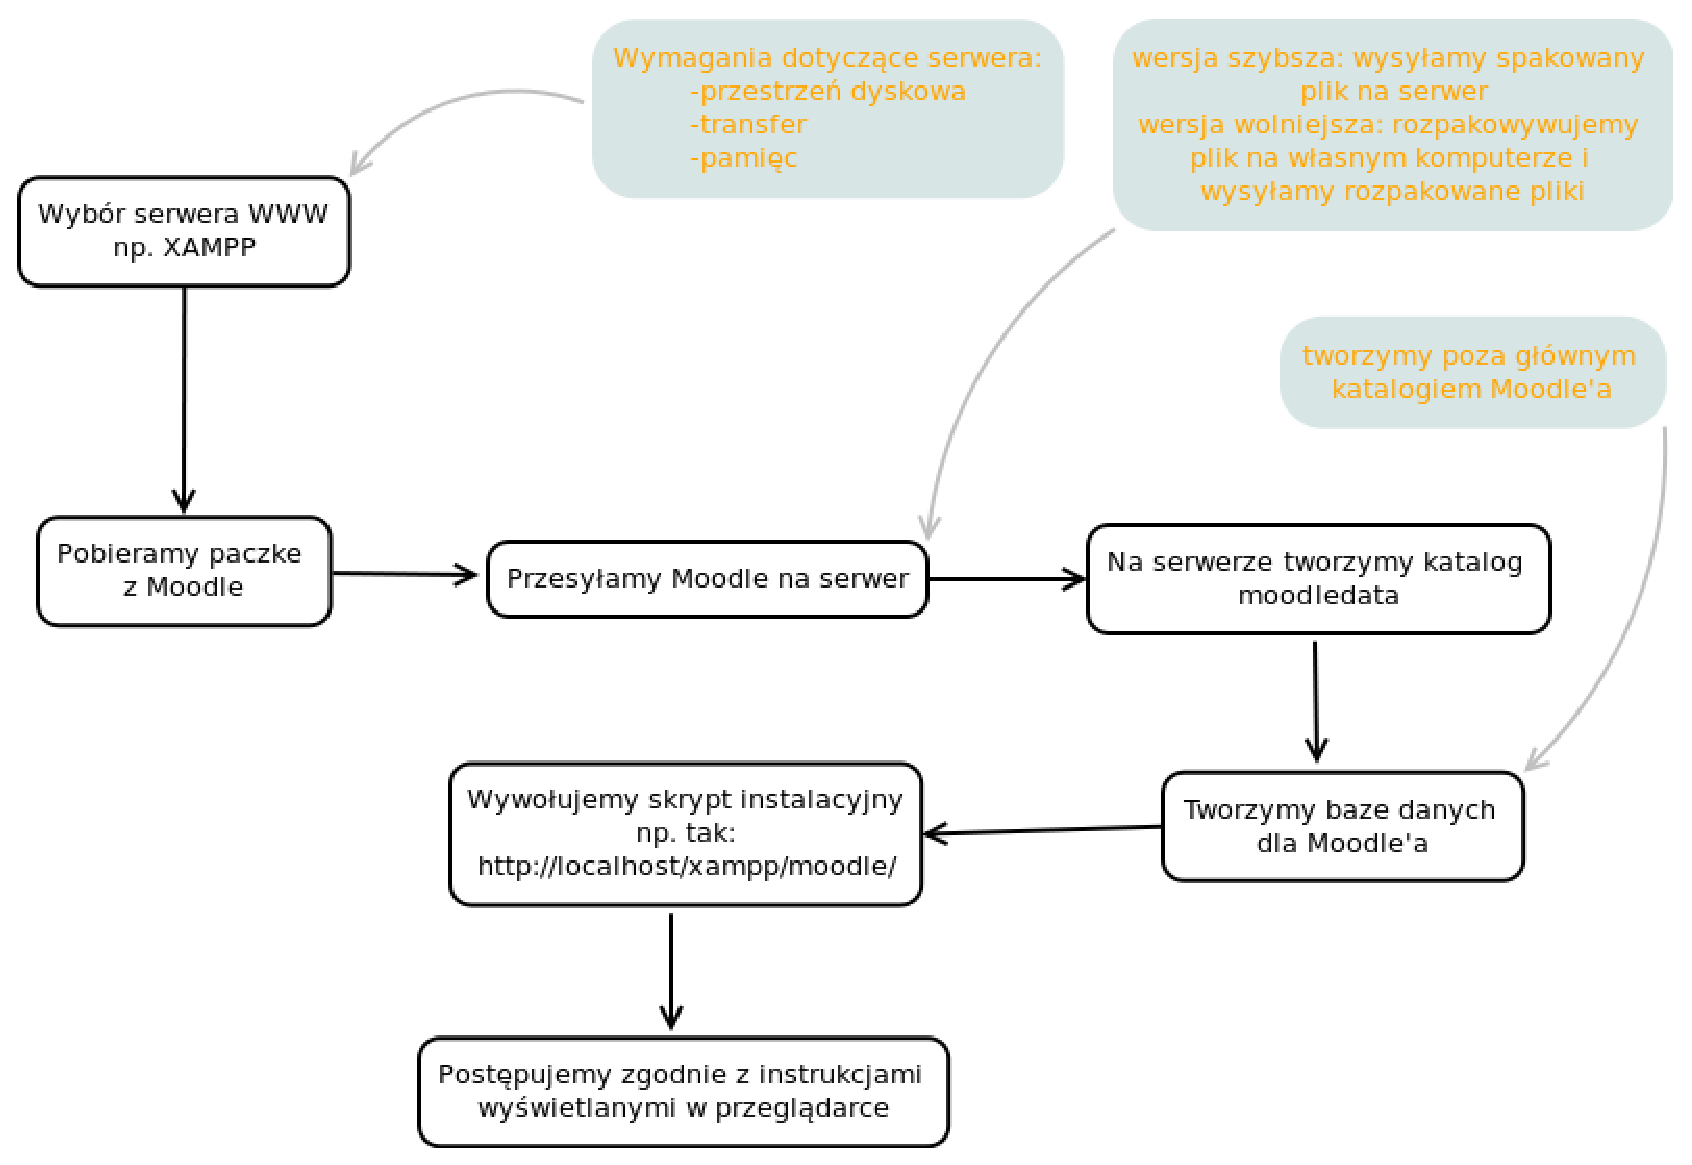
\includegraphics[width=1\textwidth]{projekt_sys//rys//instalacja.eps}
\end{figure}
\begin{figure}[!h]
	\centering
		\caption[Tworzenie kursu]{Schemat blokowy tworzenia nowego kursu} \label{rys:kurs}
		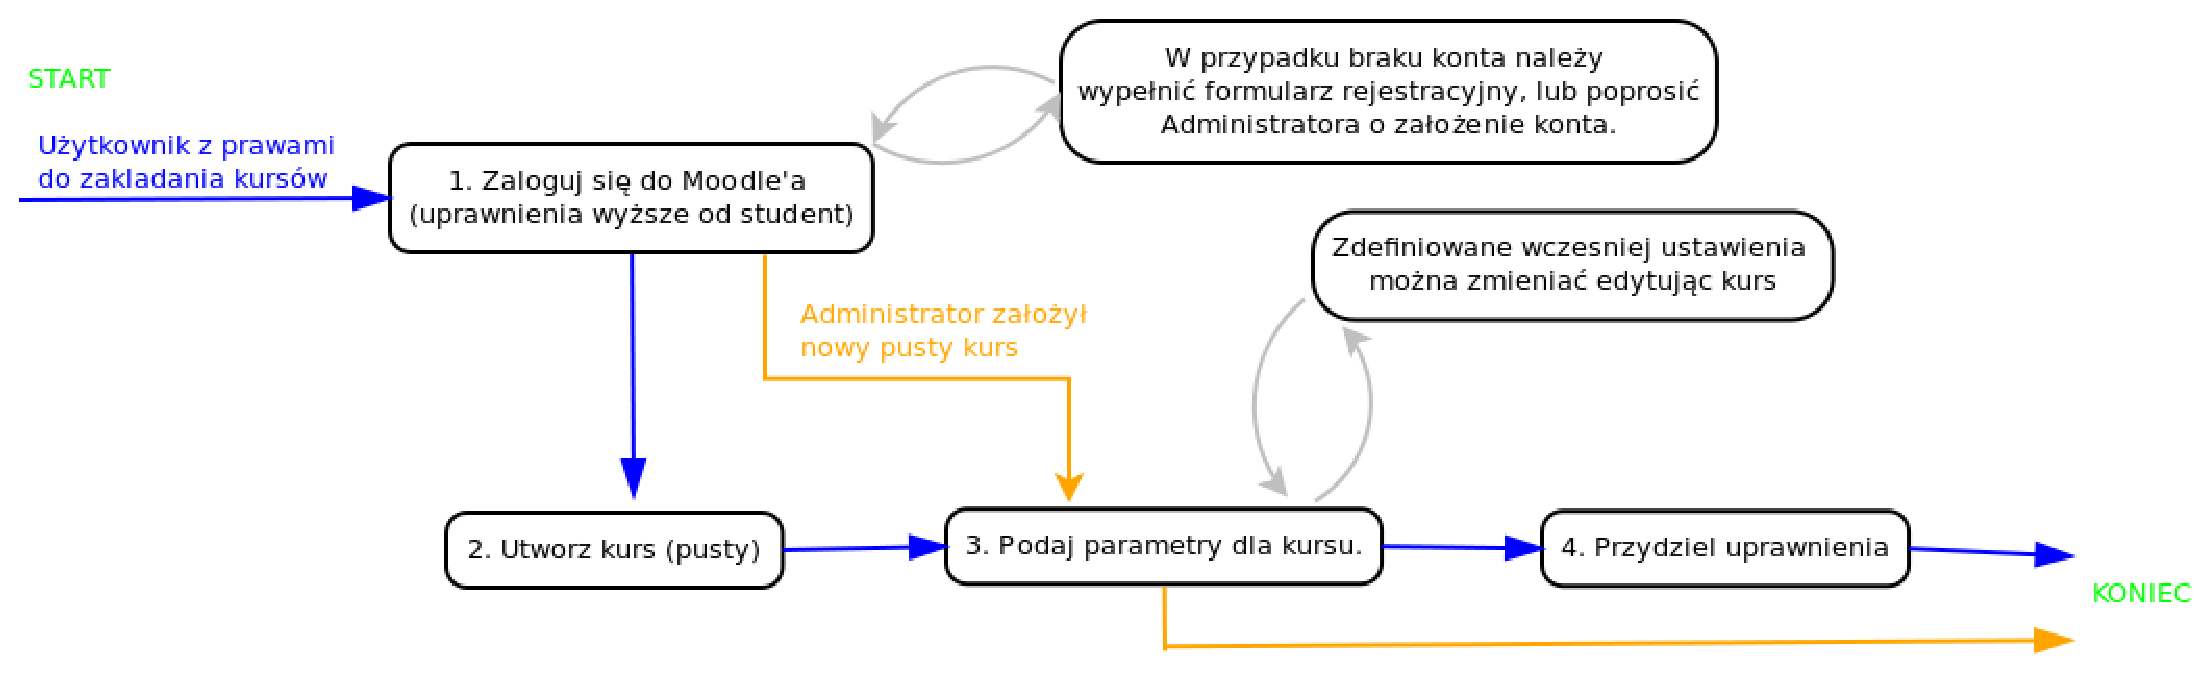
\includegraphics[width=1\textwidth]{projekt_sys//rys//nowy_kurs.eps}
\end{figure}
